% Settings for the default beamer theme
\documentclass[english, aspectratio=169]{beamer}
\usepackage[T1]{fontenc}
\usepackage[utf8]{inputenc}
\usepackage{tabularx}
\usepackage{babel}
\usepackage{hyperref}
\usepackage[ruled,vlined]{algorithm2e}
\SetAlgorithmName{Algoritmus}{algoritmus}{List of Algorithms}
\setcounter{secnumdepth}{3}
\setcounter{tocdepth}{3}

\makeatletter

\newcommand\makebeamertitle{\frame{\maketitle}}

% (ERT) argument for the TOC
\AtBeginDocument{%
  \let\origtableofcontents=\tableofcontents
  \def\tableofcontents{\@ifnextchar[{\origtableofcontents}{\gobbletableofcontents}}
  \def\gobbletableofcontents#1{\origtableofcontents}
}

% Theme settings
\usetheme{Frankfurt}
\usecolortheme{default}
\usefonttheme[onlymath]{serif}

% Template settings
\setbeamertemplate{navigation symbols}{}
\setbeamertemplate{blocks}[rounded][shadow=false]
\setbeamertemplate{title page}[default][colsep=-4bp, rounded=true, shadow=false]
\makeatother

% Define a custom darker red color
\definecolor{DarkerRed}{RGB}{139,0,0} % Adjust the RGB values as needed

% Use the newly defined color in Beamer theme elements
\setbeamercolor{structure}{fg=DarkerRed} % Changes basic structural elements to Darker Red
\setbeamercolor{title in head/foot}{bg=DarkerRed} % Changes the title in header/footer to Darker Red


\begin{document}

% Title page
\section{A gépi tanulás kihívásai}
\title[]{Üzleti Elemzések Módszertana}
\subtitle{3. Gyakorlat: Regularizált modellek}
\author[Kuknyó Dániel]{Kuknyó Dániel\\Budapesti Gazdasági Egyetem}
\date{2023/24\\2.félév}
\makebeamertitle

% Table of contents slide
\begin{frame}
\tableofcontents{}
\end{frame}

% Table of contents of the current section
\begin{frame}
\tableofcontents[currentsection]
\end{frame}

\begin{frame}{Nincs ingyen ebéd}
\begin{columns}
\begin{column}{.5\textwidth}
Ez az elv azt sugallja, hogy egy algoritmus, amely egyes feladatokon jól teljesít, nem feltétlenül fog ugyanolyan jól működni más feladatokon. \textbf{Nincs egyetemesen optimális algoritmus minden lehetséges problémára}. Ennek következményei:
\begin{itemize}
	\item Az algoritmusokat szükséges specializálni
	\item Az egyes feladatokon össze kell hasonlítani különböző modellek teljesítményét
	\item Nincs egyetemes megoldás egyetlen problémára
\end{itemize}
\end{column}
\begin{column}{.5\textwidth}
\begin{center}

\includegraphics[width=7cm, height=7cm, keepaspectratio]{images/regularization_1.png}
\end{center}
\end{column}
\end{columns}
\end{frame}

\begin{frame}{Nem reprezentatív vagy hiányos adatok}
\only<1>{\begin{columns}
\begin{column}{.5\textwidth}
A diagramon az egy főre jutó GDP és az emberek életükkel való elégedettsége látható. A mintában nem szerepelnek a gazdagabb és szegényebb országok. Ebben az esetben a becsült modell:
\begin{block}{}
\vspace{-0.2cm}
\[
\hat{y} = 4.85 + 4.91 \cdot 10^{-5} \cdot x
\]
\end{block}
Tehát $\theta = \left[ \theta_0, \theta_1 \right] = \left[ 4.85, 4.91 \cdot 10^{-5} \right]$
\end{column}
\begin{column}{.5\textwidth}
\begin{center}
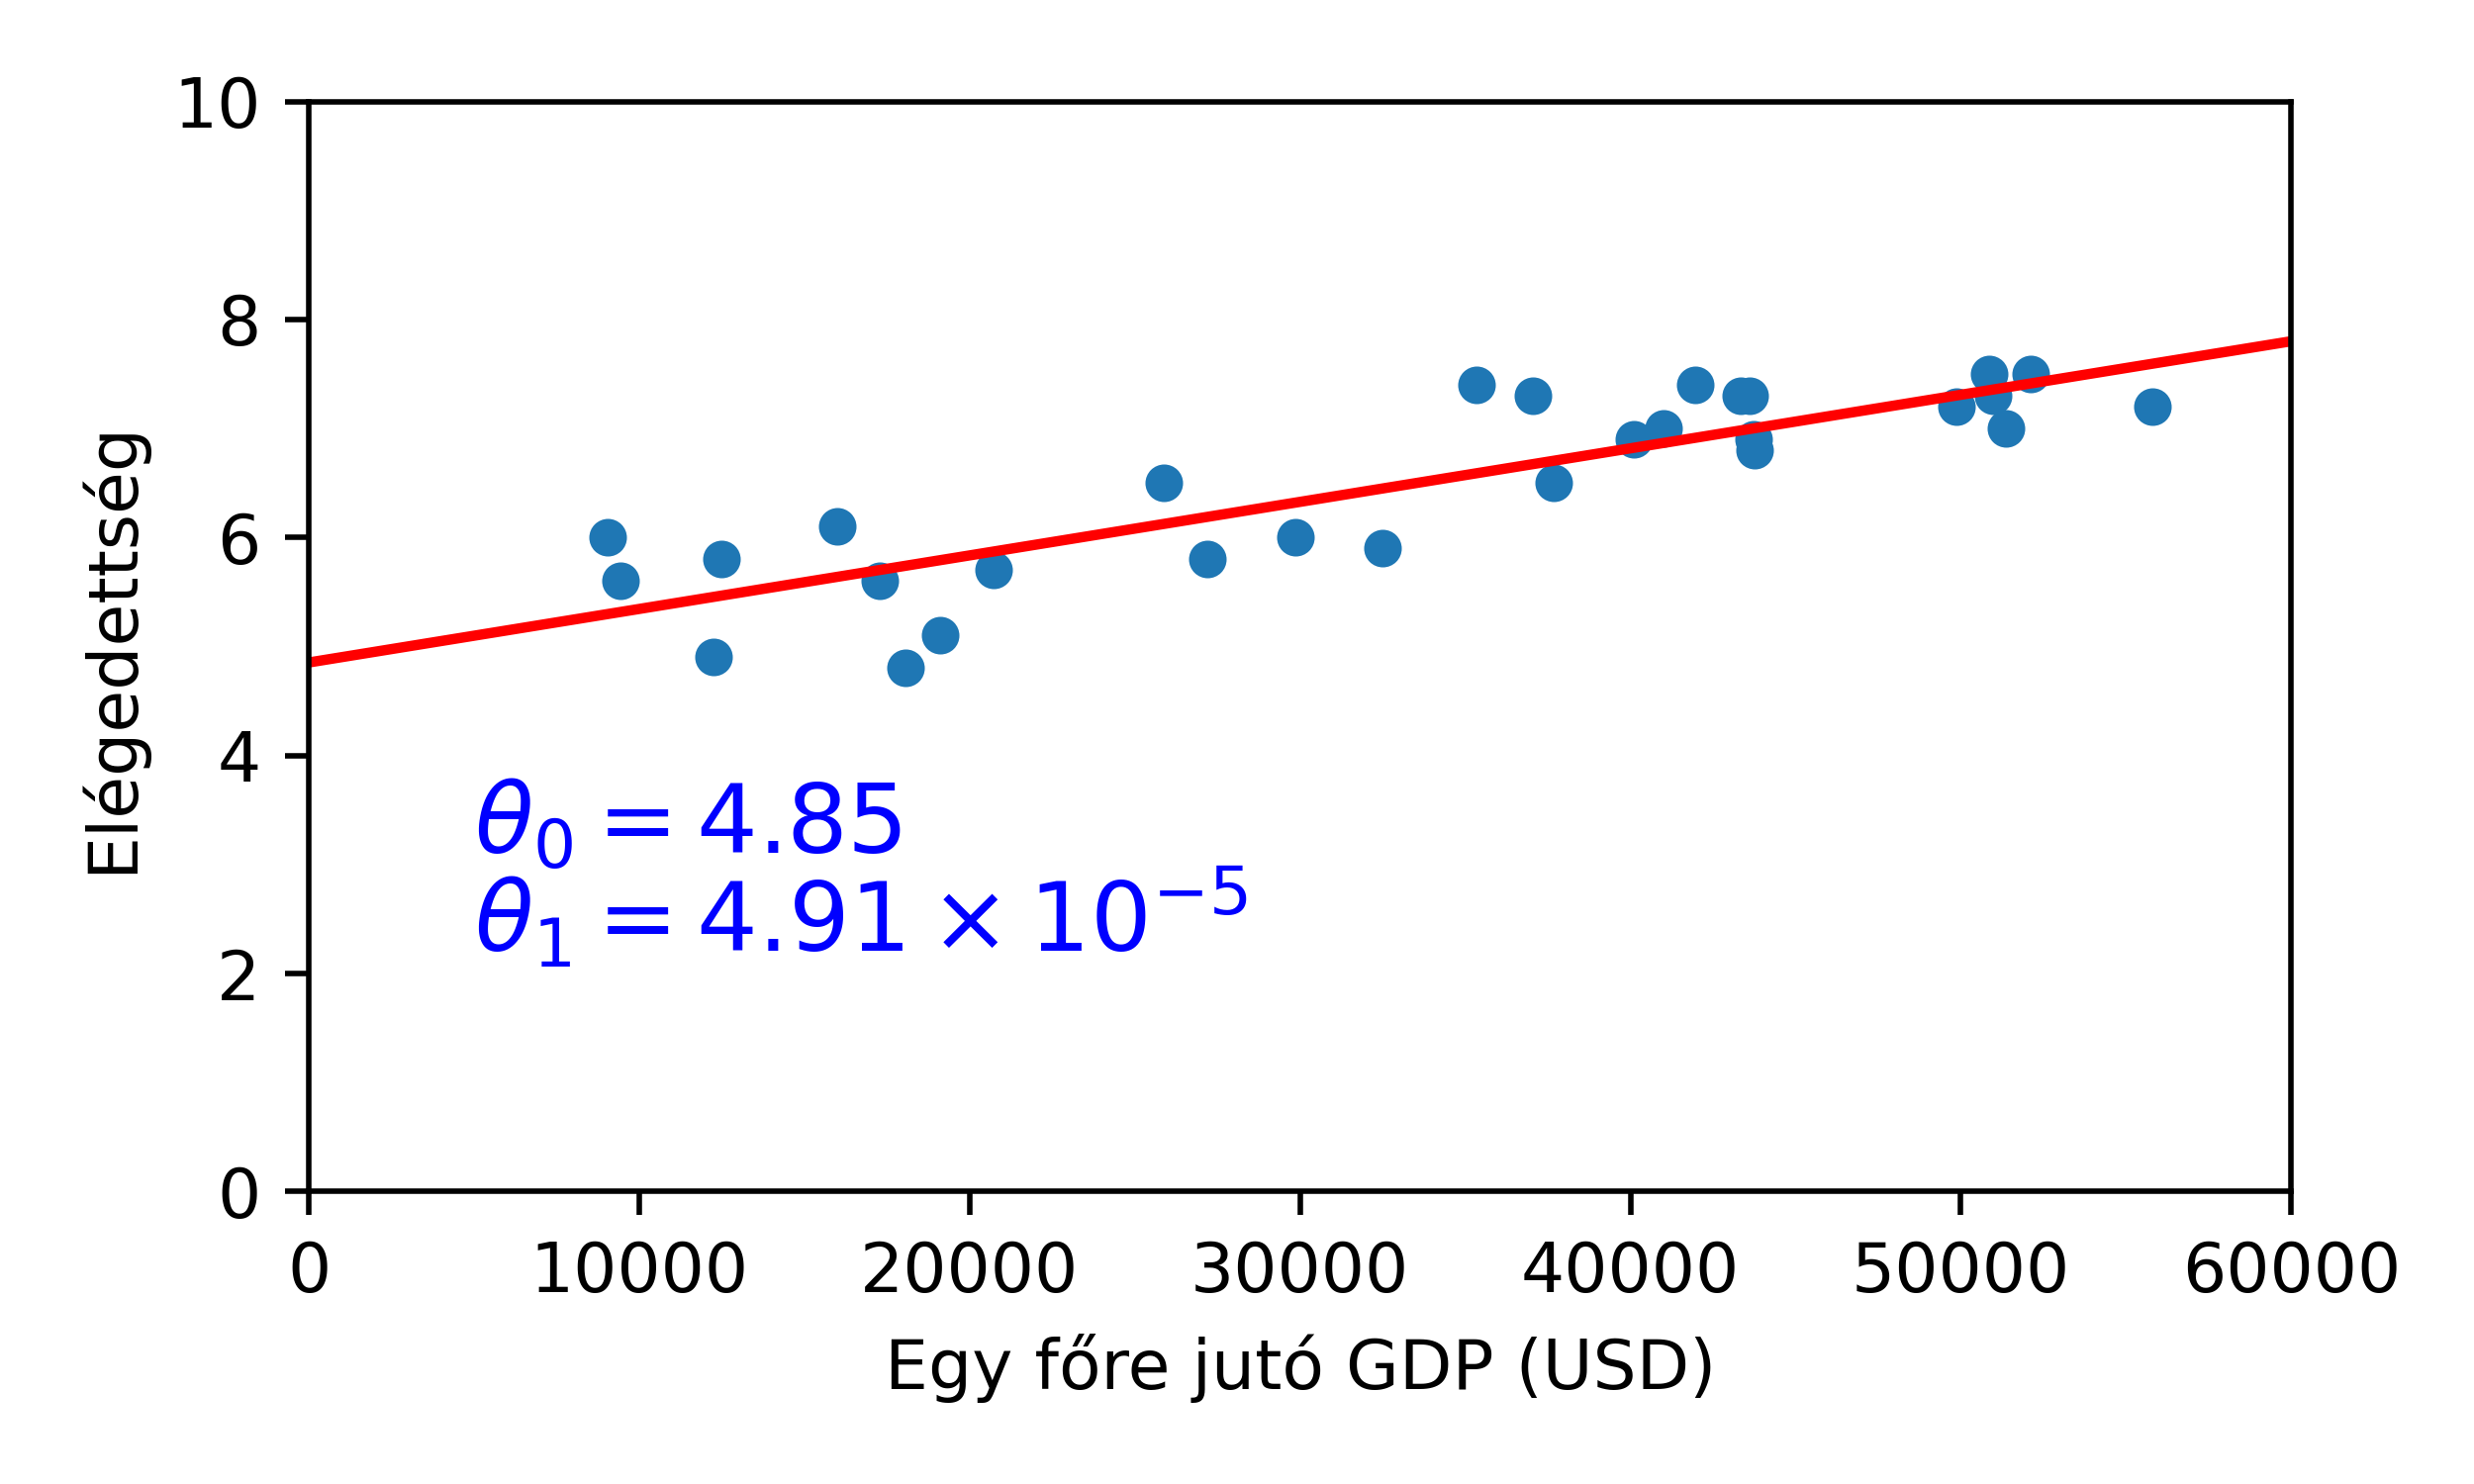
\includegraphics[width=7cm, height=7cm, keepaspectratio]{images/regularization_2.png}
\end{center}
\end{column}
\end{columns}}
\only<2>{\begin{columns}
\begin{column}{.5\textwidth}
Érdemes megfigyelni mi történik, ha több ország is hozzáadódik a mintához, amik eddig nem szerepelnek benne. Az \textbf{illesztett modell egy szignifikáns változáson megy keresztül}:
\begin{block}{}
\vspace{-0.2cm}
\[
\hat{y} = 5.8 + 2.31 \cdot 10^{-5}
\]
\end{block}
\par\smallskip
A modell változása annak a következménye, hogy az előző minta \textbf{nem volt megfelelően reprezentatív} az összes országra való tekintettel.
\end{column}
\begin{column}{.5\textwidth}
\begin{center}
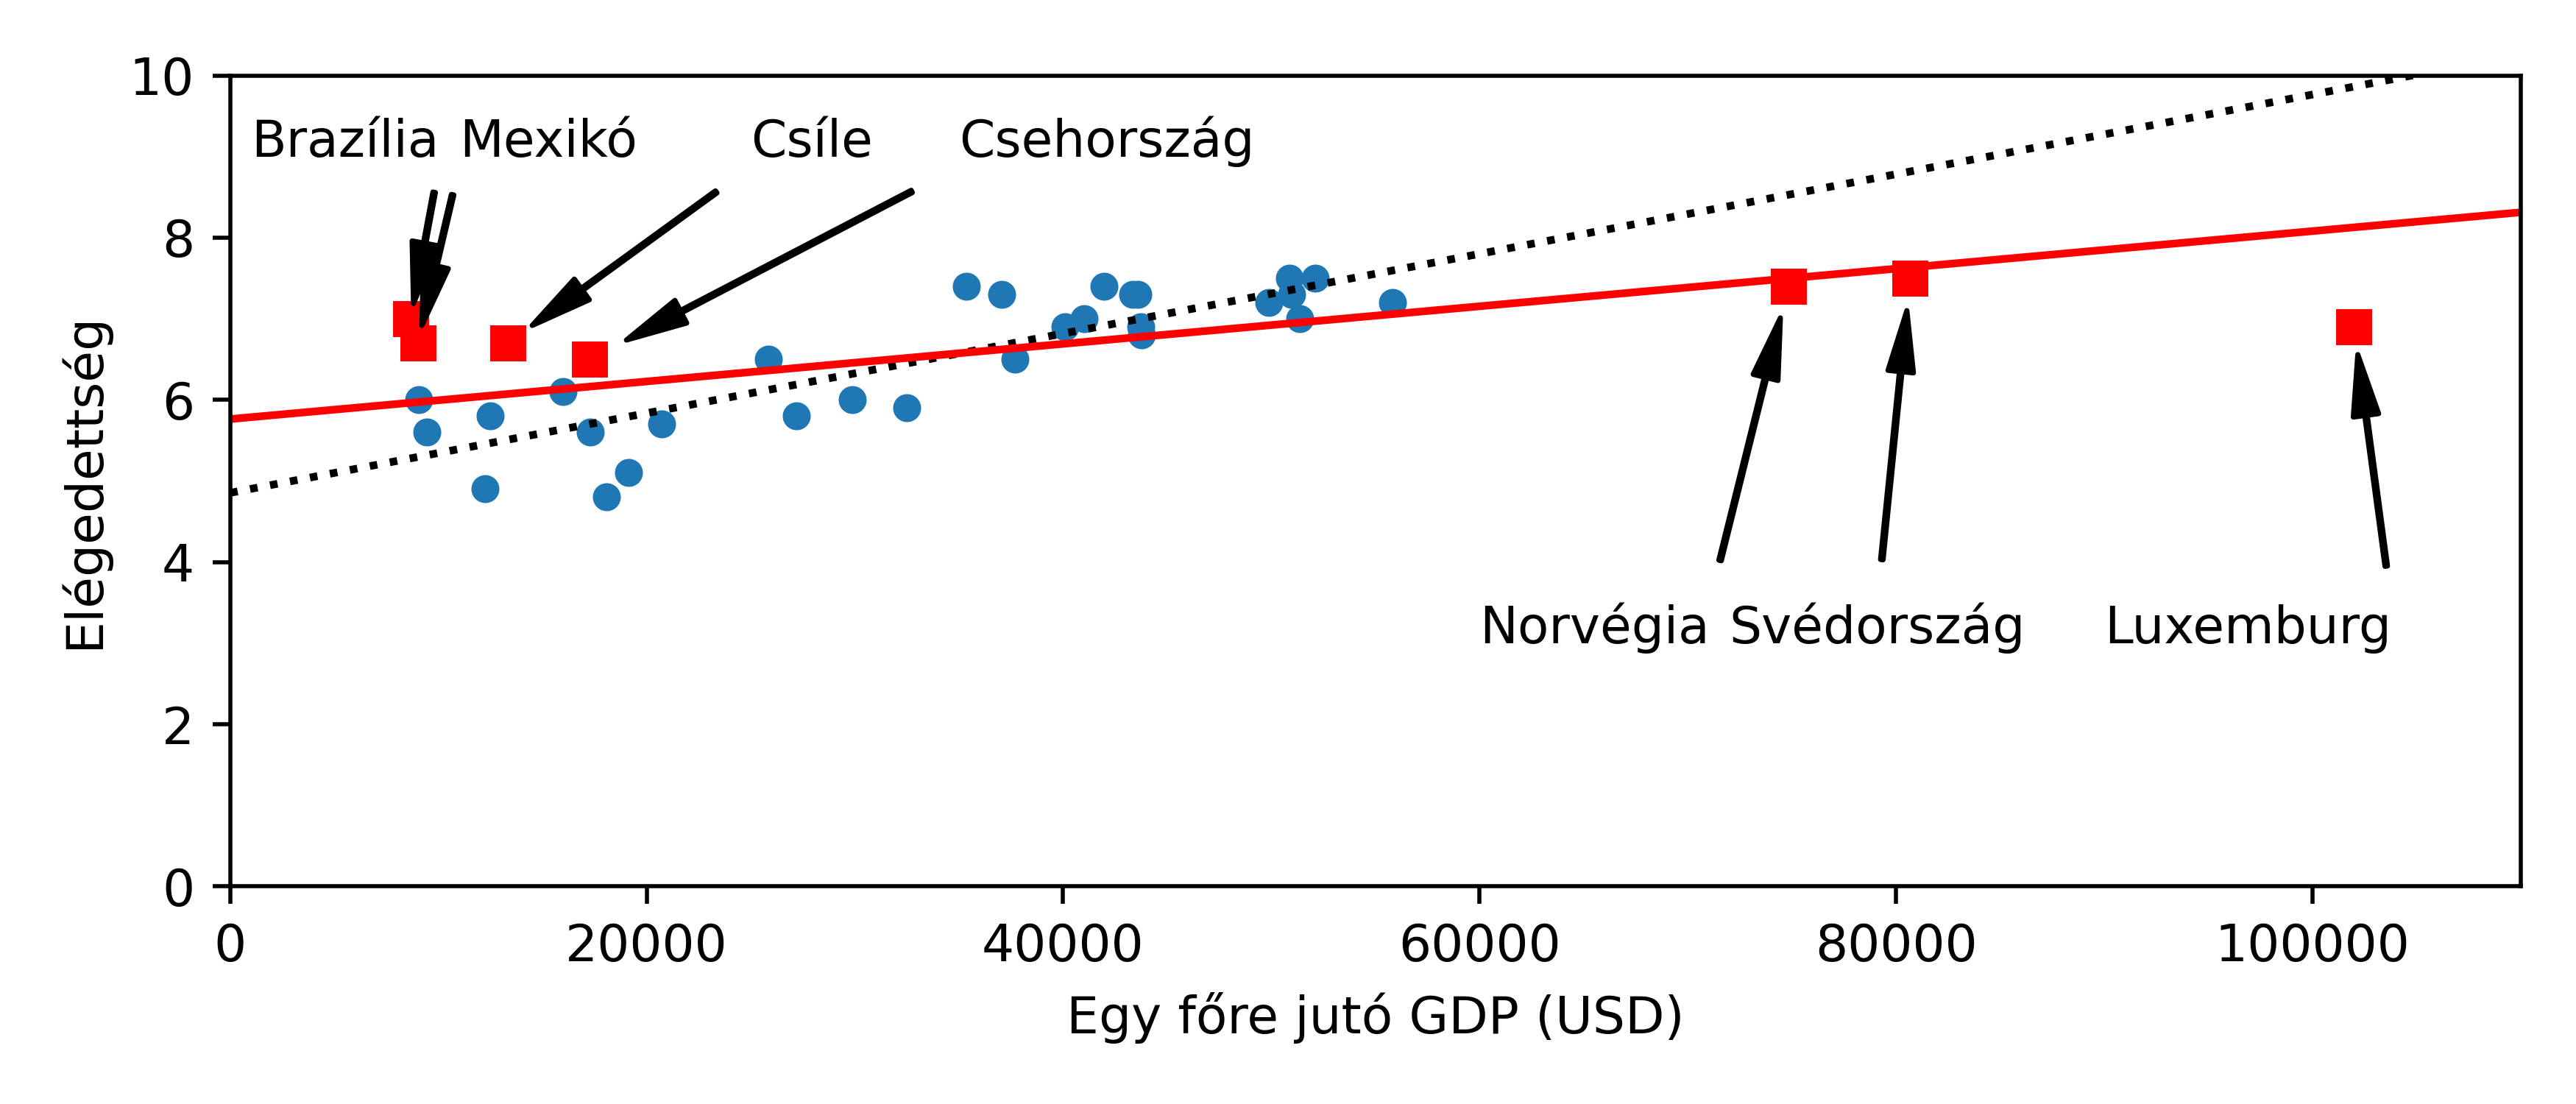
\includegraphics[width=7cm, height=7cm, keepaspectratio]{images/regularization_3.png}
\end{center}
\end{column}
\end{columns}}
\end{frame}

\begin{frame}{A túltanulás problémája}
\begin{columns}
\begin{column}{.5\textwidth}
A túltanulás onnan ered, hogy az \textbf{illesztett modellnek túlságosan magas a szabadságfoka}, vagy túl sok iteráción keresztül folyik a tanítás.\par\smallskip
A túltanult modell \textbf{nagyon pontosan képes illeszkedni a tanító adatokra}, de nem fog jól teljesíteni a teszt adatokon. Emiatt rossz általánosító képességekkel fog rendelkezni. 
\end{column}
\begin{column}{.5\textwidth}
\begin{center}
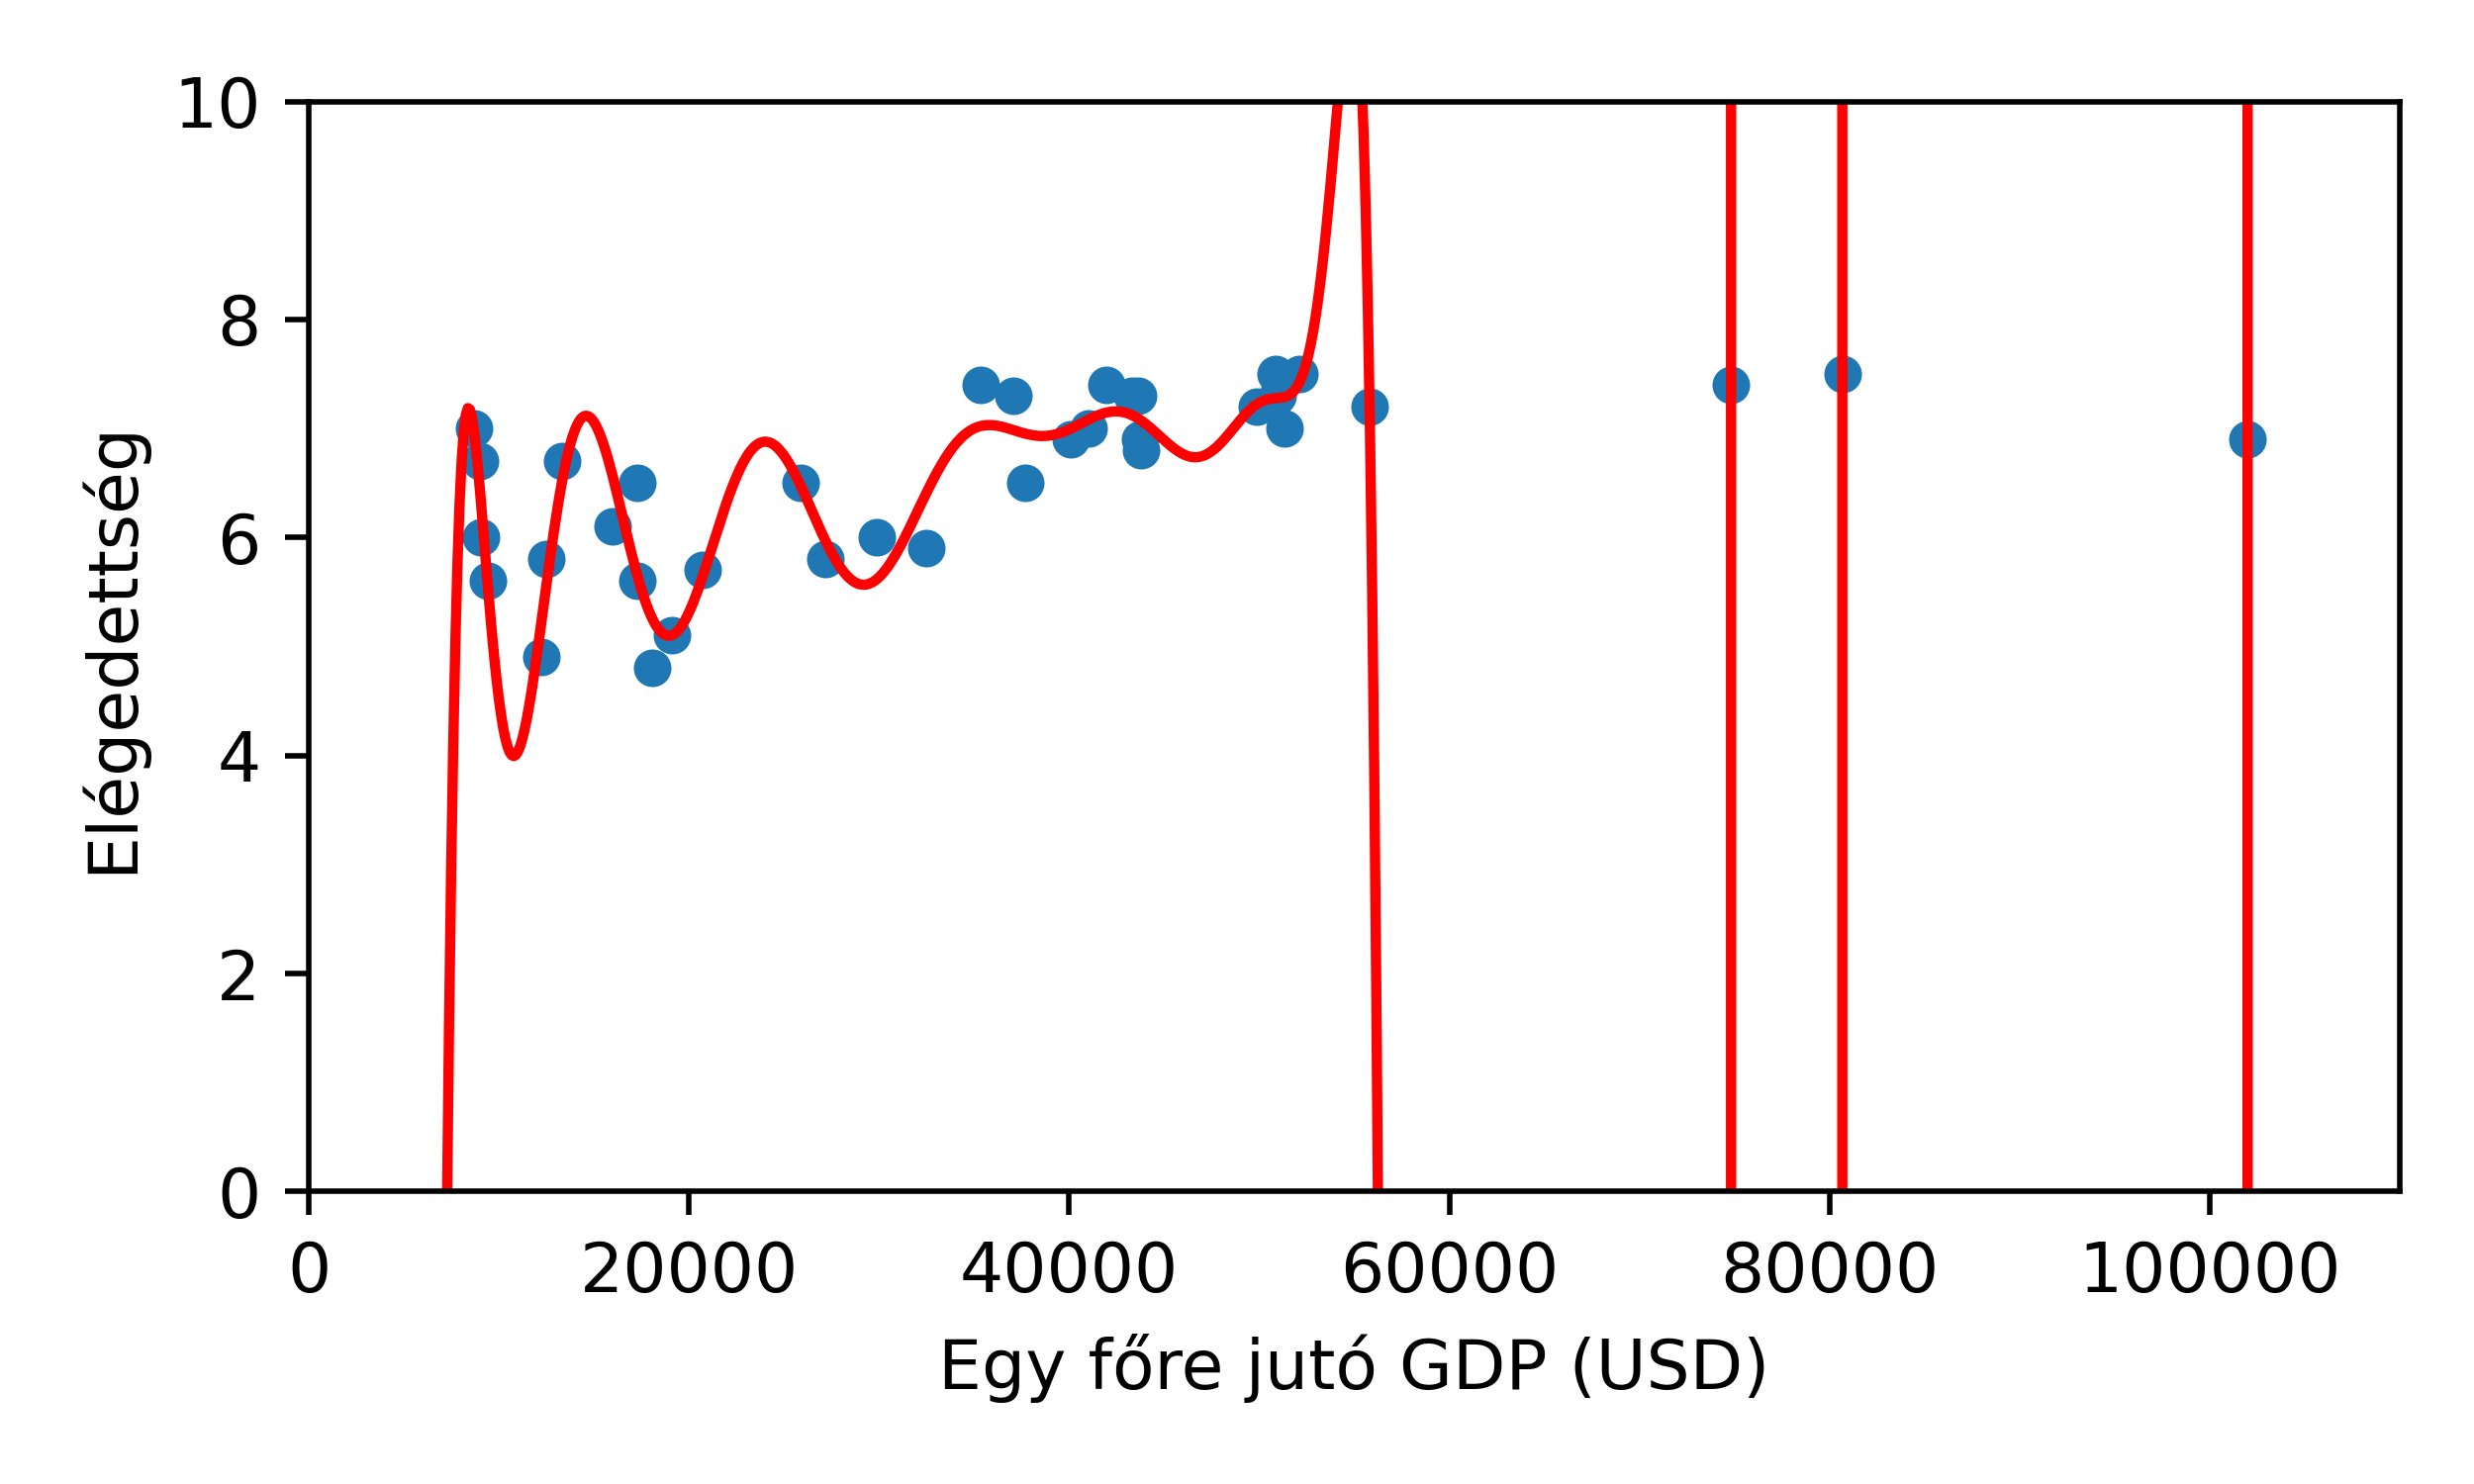
\includegraphics[width=7cm, height=7cm, keepaspectratio]{images/regularization_4.png}
\end{center}
\end{column}
\end{columns}
\end{frame}

\section{Polinomiális regresszió}

\begin{frame}
\tableofcontents[currentsection]
\end{frame}

\begin{frame}{Polinomiális adatok}
\begin{columns}
\begin{column}{.5\textwidth}
\only<1>{A valóságban nagyon kevés olyan adathalmaz létezik, amik leírhatók egy lineáris modellel\par\smallskip
Ennek megfelelően szükség van komplexebb, nagyobb paraméterszámmal rendelkező modellekre, mint a polinomiális regresszor. modellek.}
\only<2>{\begin{block}{Polinomiális regresszor modell}
Olyan típusú regressziós analízis, ahol a kapcsolat az $x$ és $y$ változók között \textbf{polinomok segítségével van modellezve}.\par\medskip
A modell magában foglalja \textbf{a független változók magasabb rendű hatványait} és azok interakcióit is. Általános formája:
\[
\hat{y} = \theta_0 + \theta_1x + \theta_2x^2 + \theta_3x^3 + \cdots + \theta_nx^n
\]
\end{block}}
\end{column}
\begin{column}{.5\textwidth}
\only<1>{\begin{center}
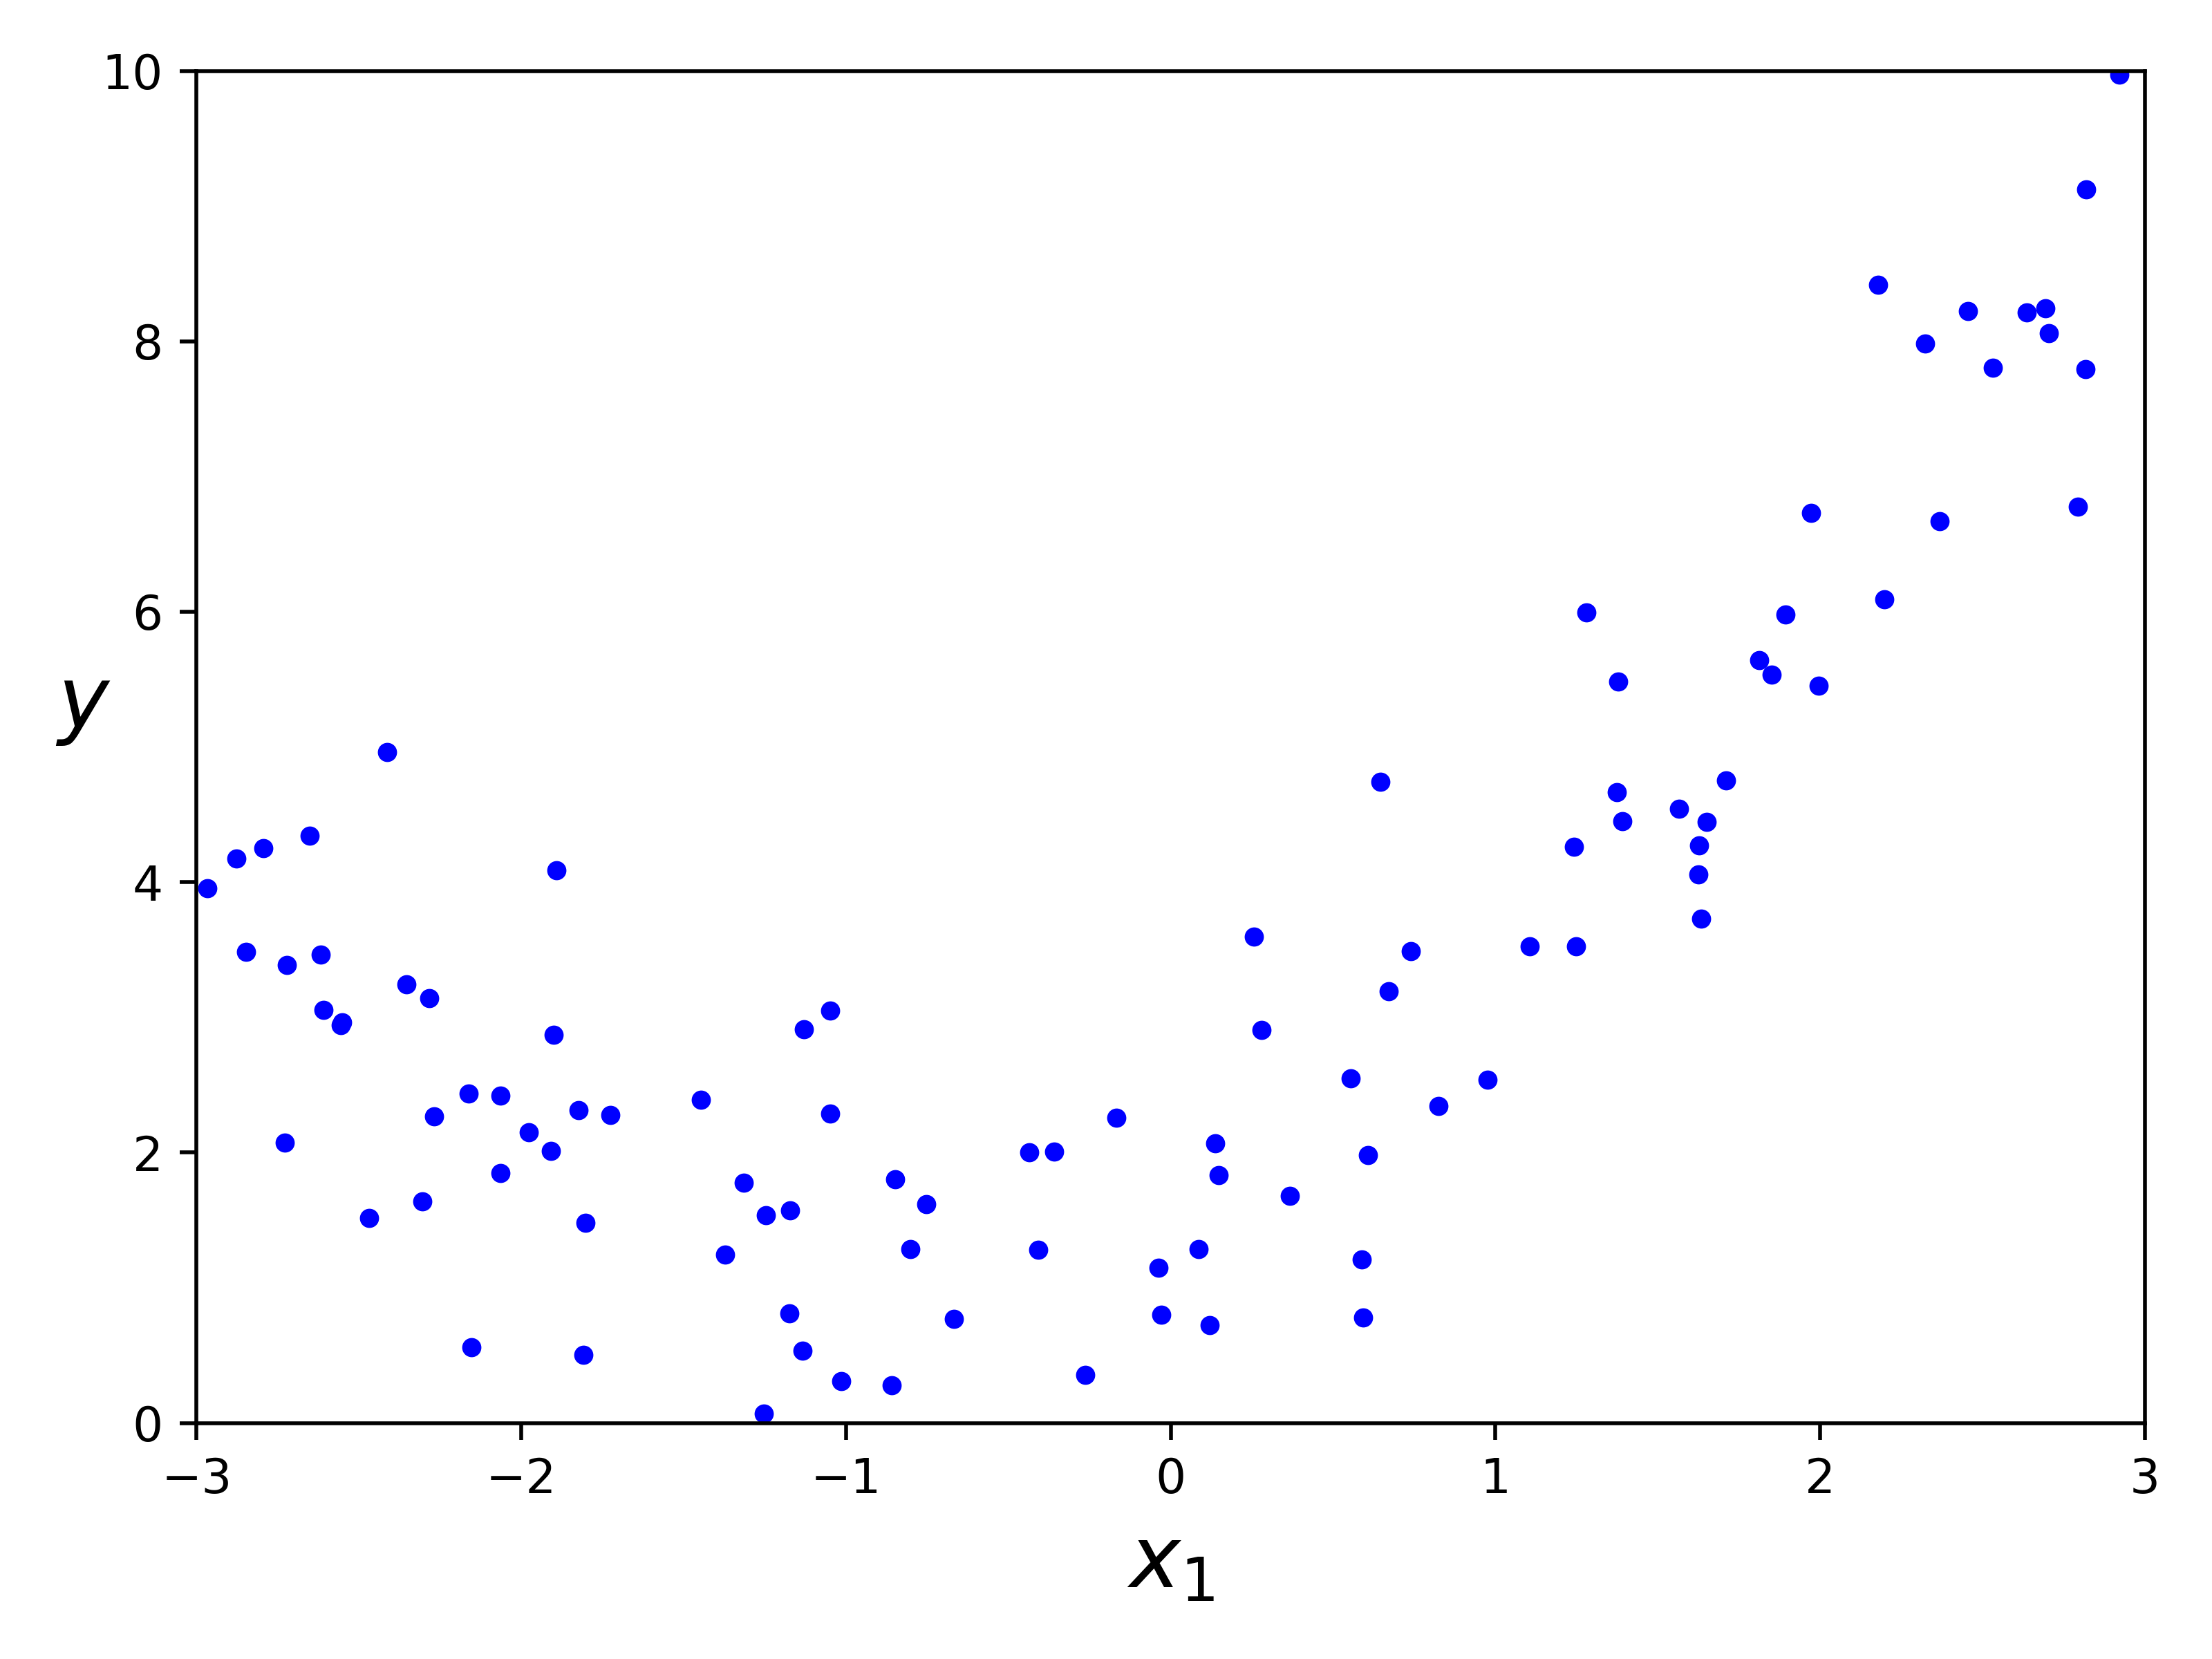
\includegraphics[width=7cm, height=7cm, keepaspectratio]{images/regularization_6.png}
\end{center}}
\only<2>{\begin{center}
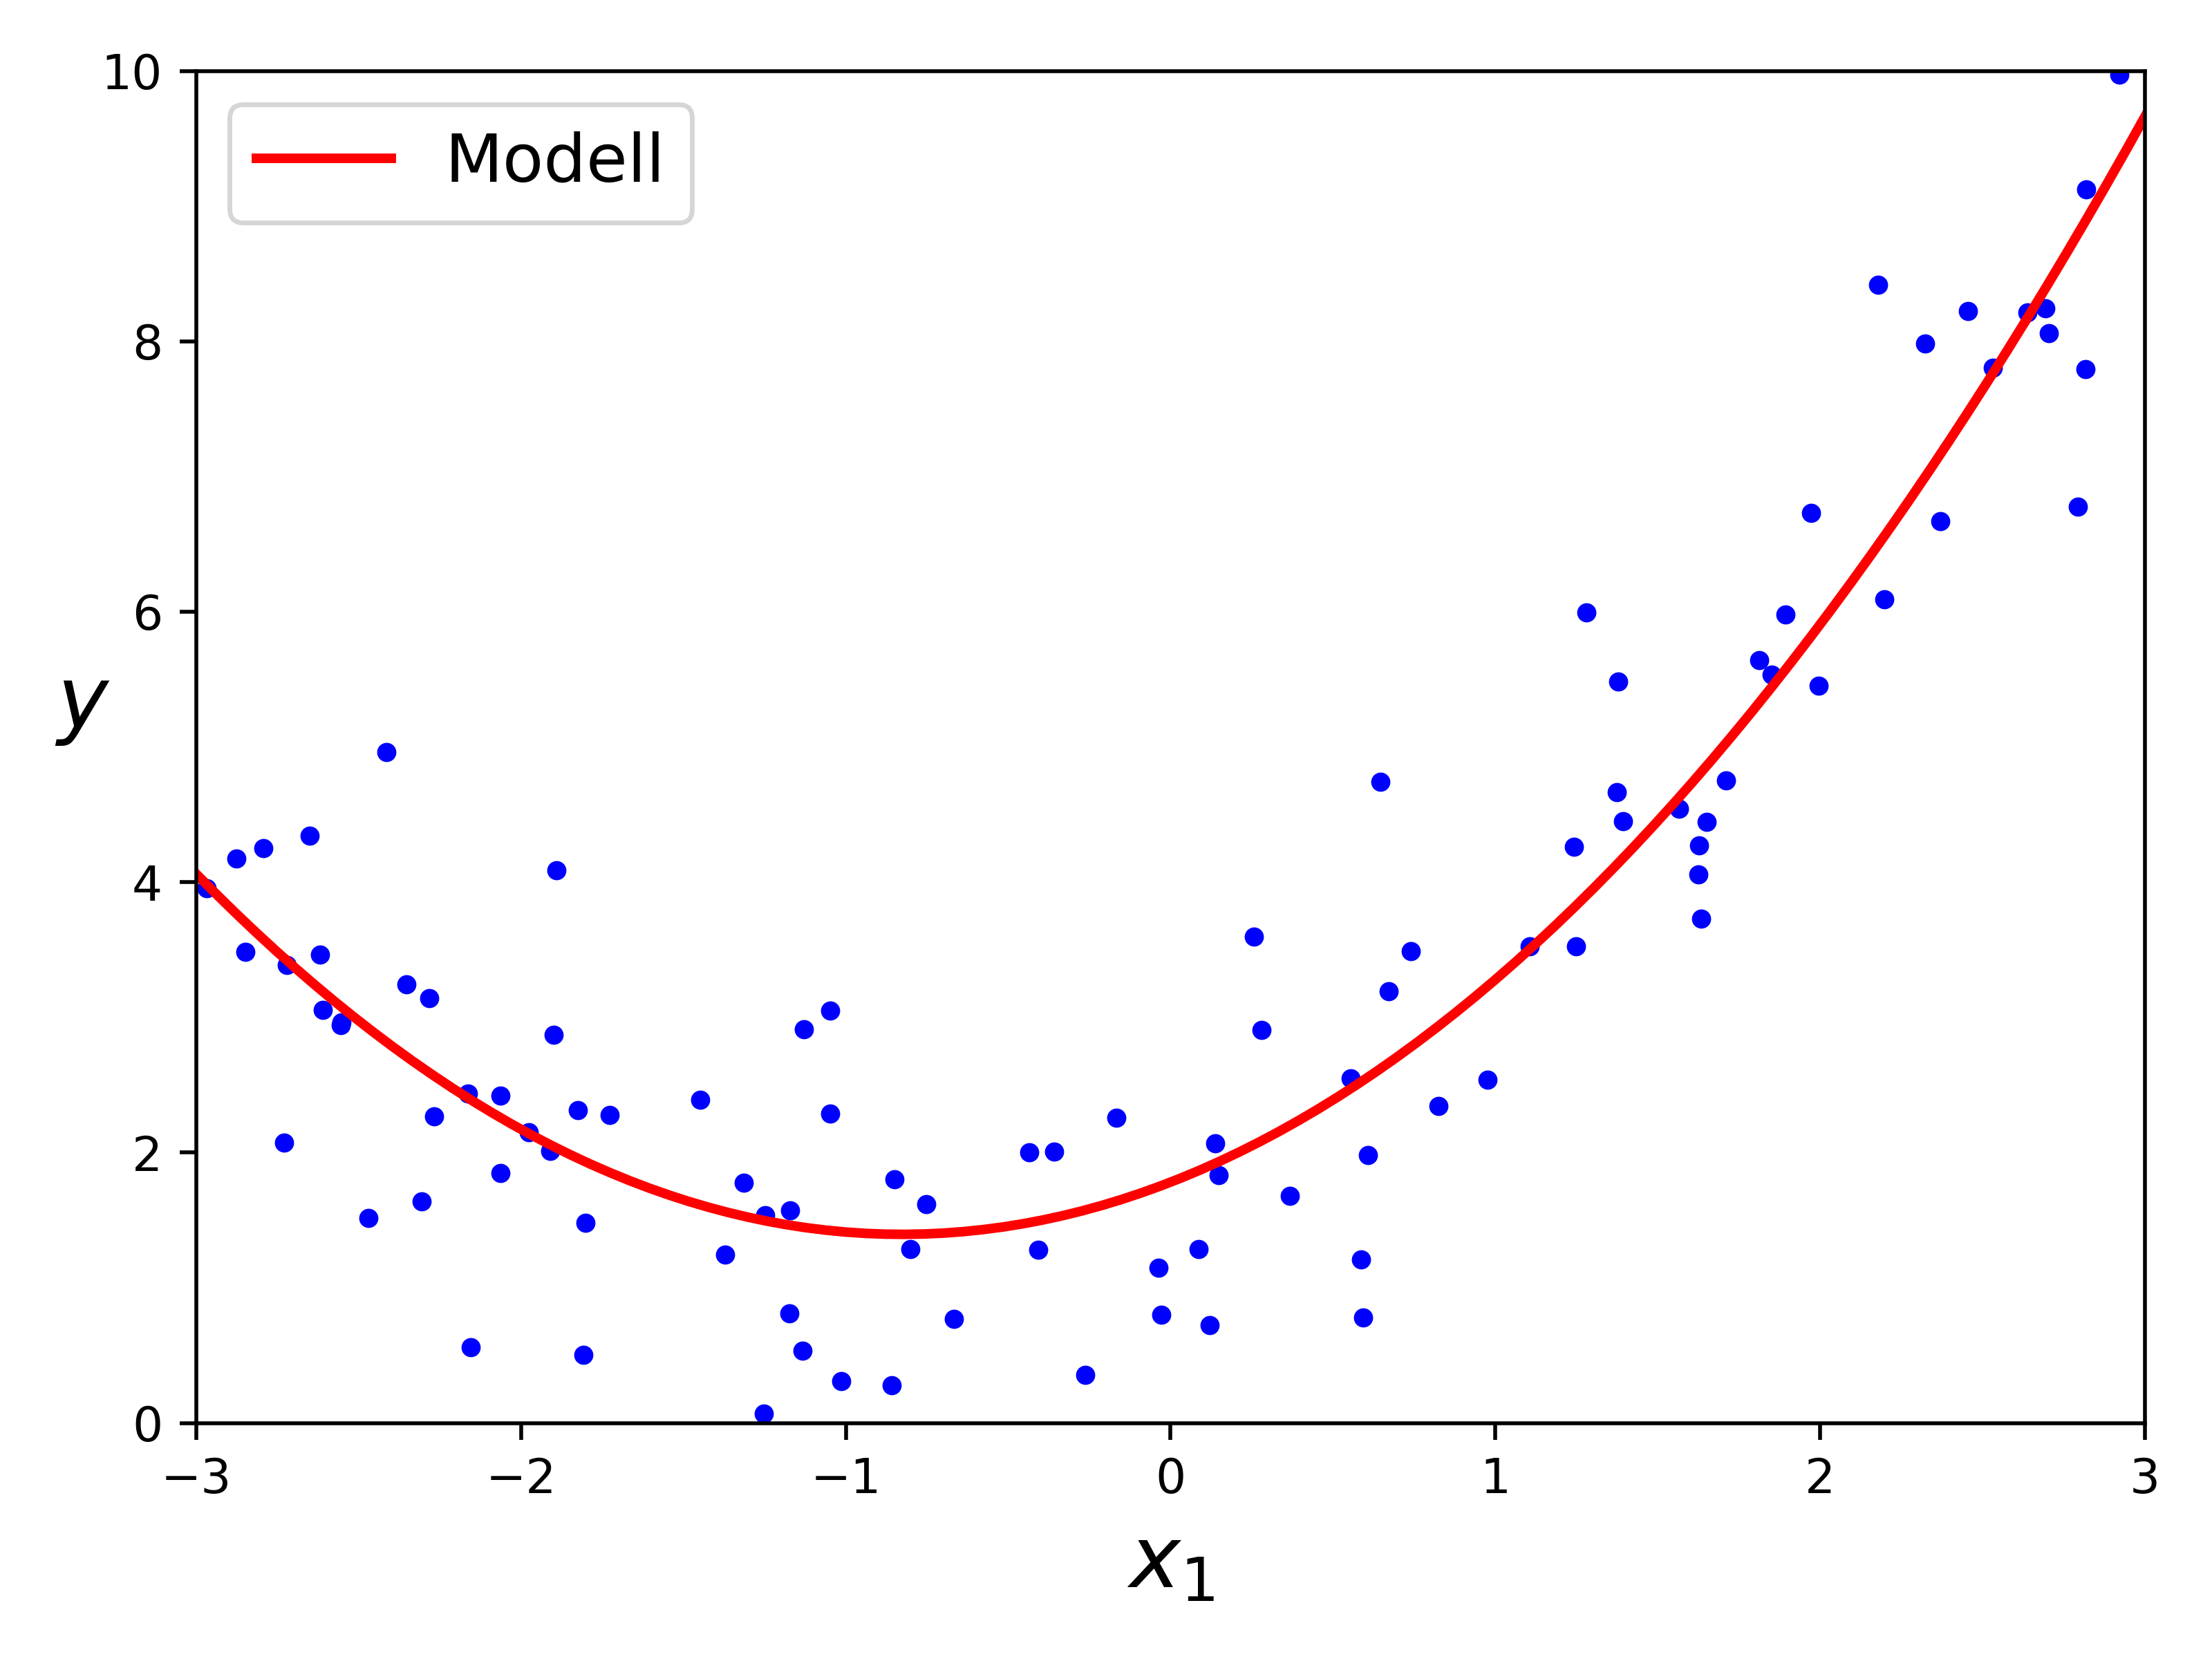
\includegraphics[width=7cm, height=7cm, keepaspectratio]{images/regularization_7.png}
\end{center}}
\end{column}
\end{columns}
\end{frame}

\begin{frame}{Tanulási görbe lineáris és polinomiális esetben}
\begin{columns}
\begin{column}{.5\textwidth}
A tanulási görbe azt mutatja meg, hogy az adott modellnek mekkora a hibája a tanító és teszt adatokon, a tanító adatok mennyiségének függvényében.\par\medskip
A polinomikus modellnek \textbf{magasabb a szabadságfoka, ezért alacsonyabb hibát képes elérni} ugyanazon az adathalmazon. Viszont ebben az esetben fennáll a túltanulás kockázata. 
\end{column}
\begin{column}{.5\textwidth}
\begin{center}
\includegraphics<1>[width=7cm, height=7cm, keepaspectratio]{images/regularization_8.png}
\includegraphics<2>[width=7cm, height=7cm, keepaspectratio]{images/regularization_9.png}
\end{center}
\end{column}
\end{columns}
\end{frame}

\begin{frame}{Regularizáció}
\begin{block}{Regularizáció}
Gépi tanulásban és a statisztikai modellezésben egy technika, amelynek célja, hogy csökkentse a modell túlillesztését és javítsa a modell általánosító képességét új adatokra azáltal, hogy \textbf{segít a modell súlyait alacsonyan tartani}.
\end{block}
\begin{center}
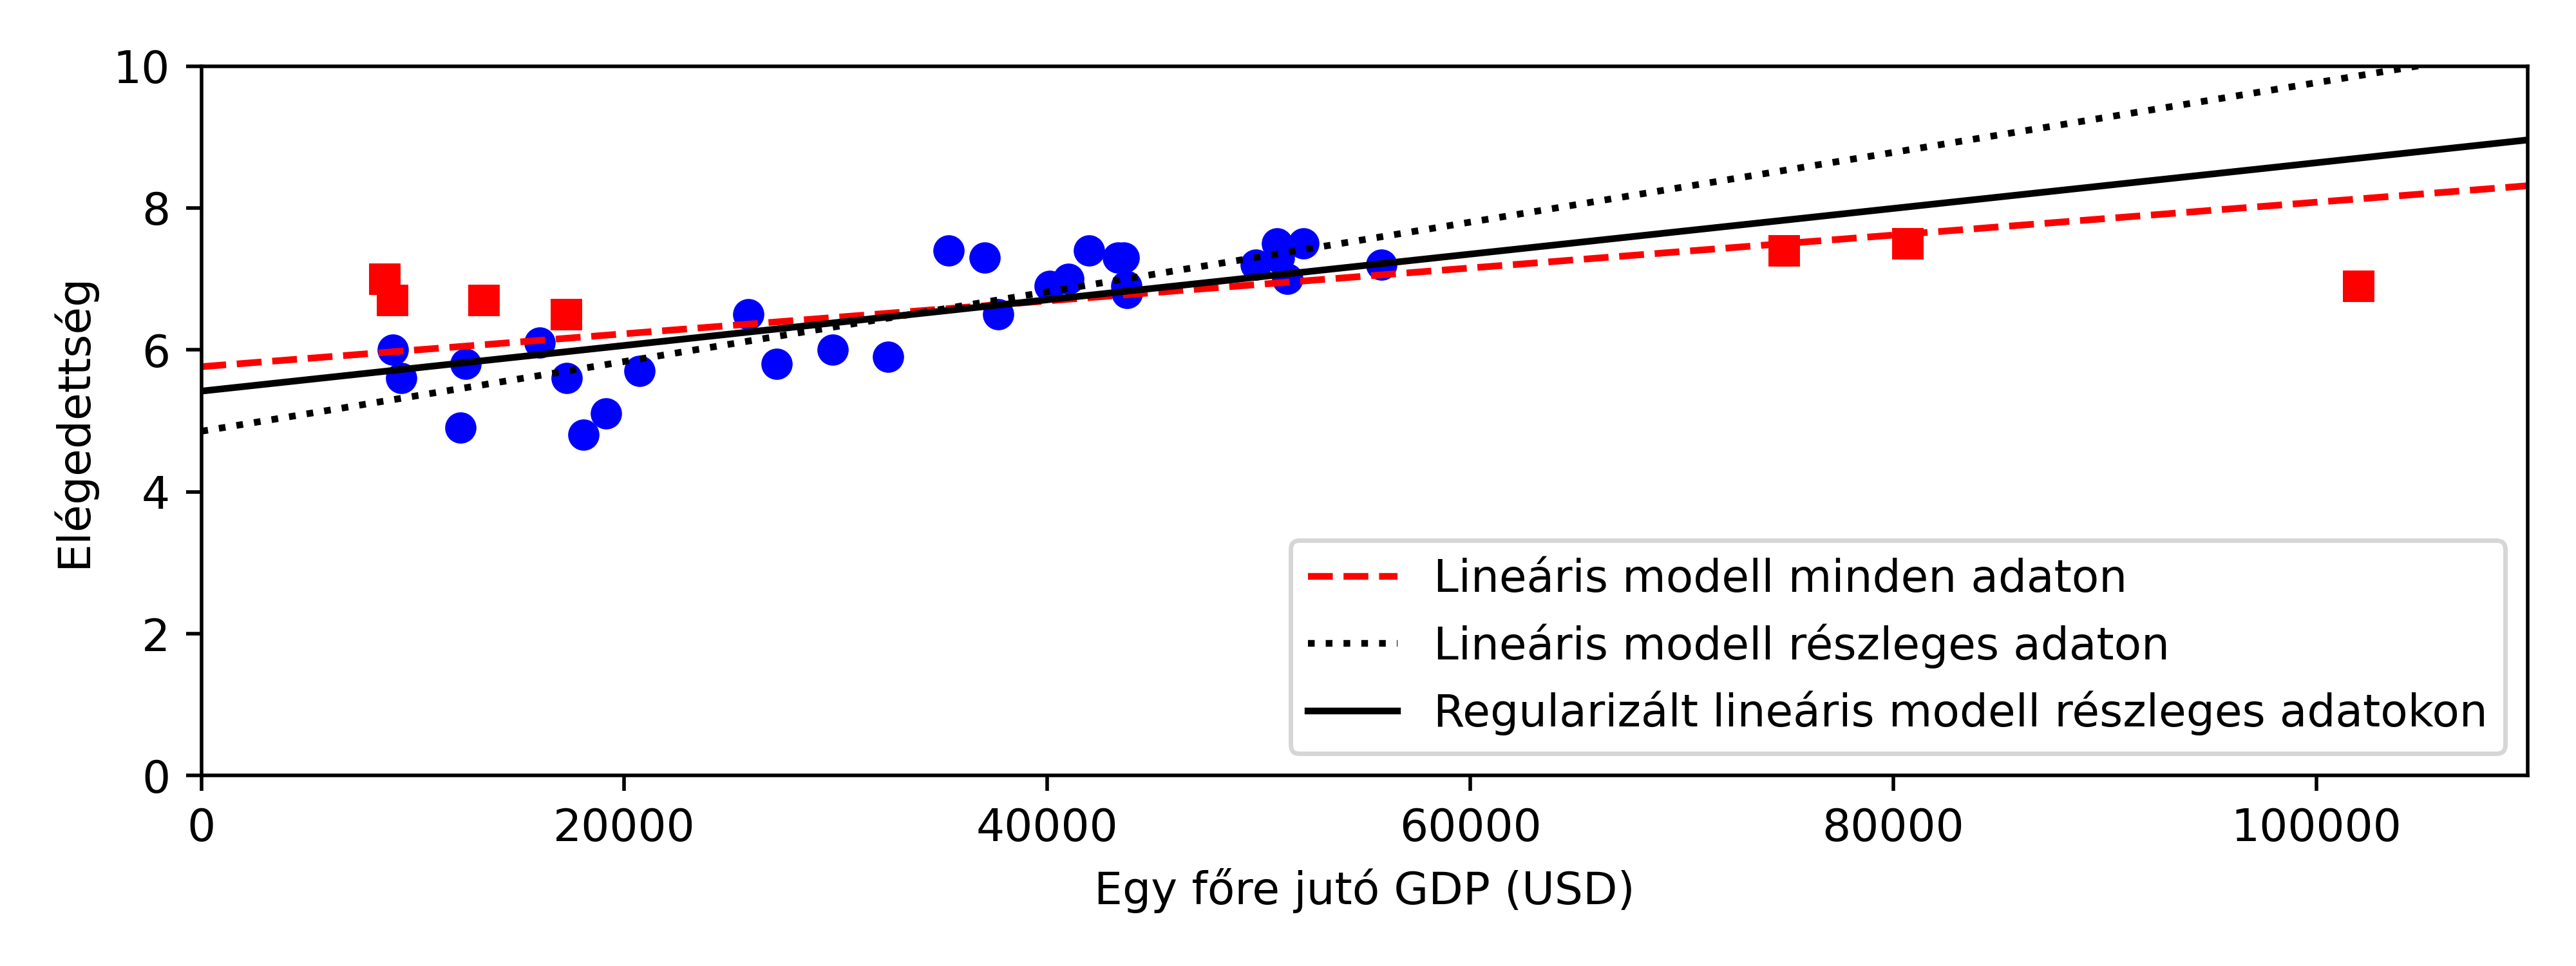
\includegraphics[width=13cm, height=7cm, keepaspectratio]{images/regularization_10.png}
\end{center}
\end{frame}

\section{Regularizált modellek}

\begin{frame}
\tableofcontents[currentsection]
\end{frame}

\begin{frame}{Ridge regresszió}
\begin{columns}
\begin{column}{.5\textwidth}
A lineáris regresszió regularizált változata, más néven Tikhonov regularizáció. Az algoritmus a függvény pontos illesztése mellett \textbf{célja a súlyokat a lehető legalacsonyabban tartan}i.\par\medskip
Ezt úgy éri el, hogy a tanítási fázisban bevezet egy \textbf{regularizációs büntetőkifejezést}, és hozzáadja a már meglévő költségfüggvényhez.
\end{column}
\begin{column}{.5\textwidth}
\begin{block}{A Ridge költségfüggvénye}
\[
J\left( \theta \right) = MSE\left( \theta \right) + \alpha \sum \theta^2
\]
Ahol: 
\begin{itemize}
	\item $MSE=\frac{1}{n} \sum_{i=1}^n \left( y_i - \hat{y}_i \right)^2$ az átlagos eltérés-négyzet
	\item $\sum \theta^2$ az $\ell_2$ norma büntetőkifejezés
	\item $\alpha$ a regularizáció mértékét adó együttható
	\item $\theta$ a paraméterek vektora
\end{itemize}
\end{block}
\end{column}
\end{columns}
\end{frame}

\begin{frame}{Ridge a gyakorlatban}
A két ábrán különböző $\alpha$ paraméterrel tanított regularizált modellek láthatók. A bal oldali diagramon lineáris modellek, a jobb oldalin pedig polinomiális függvények illeszkednek az adathalmazra. Minél nagyobb az $\alpha$, annál általánosabb az modell.\par\medskip
\begin{center}
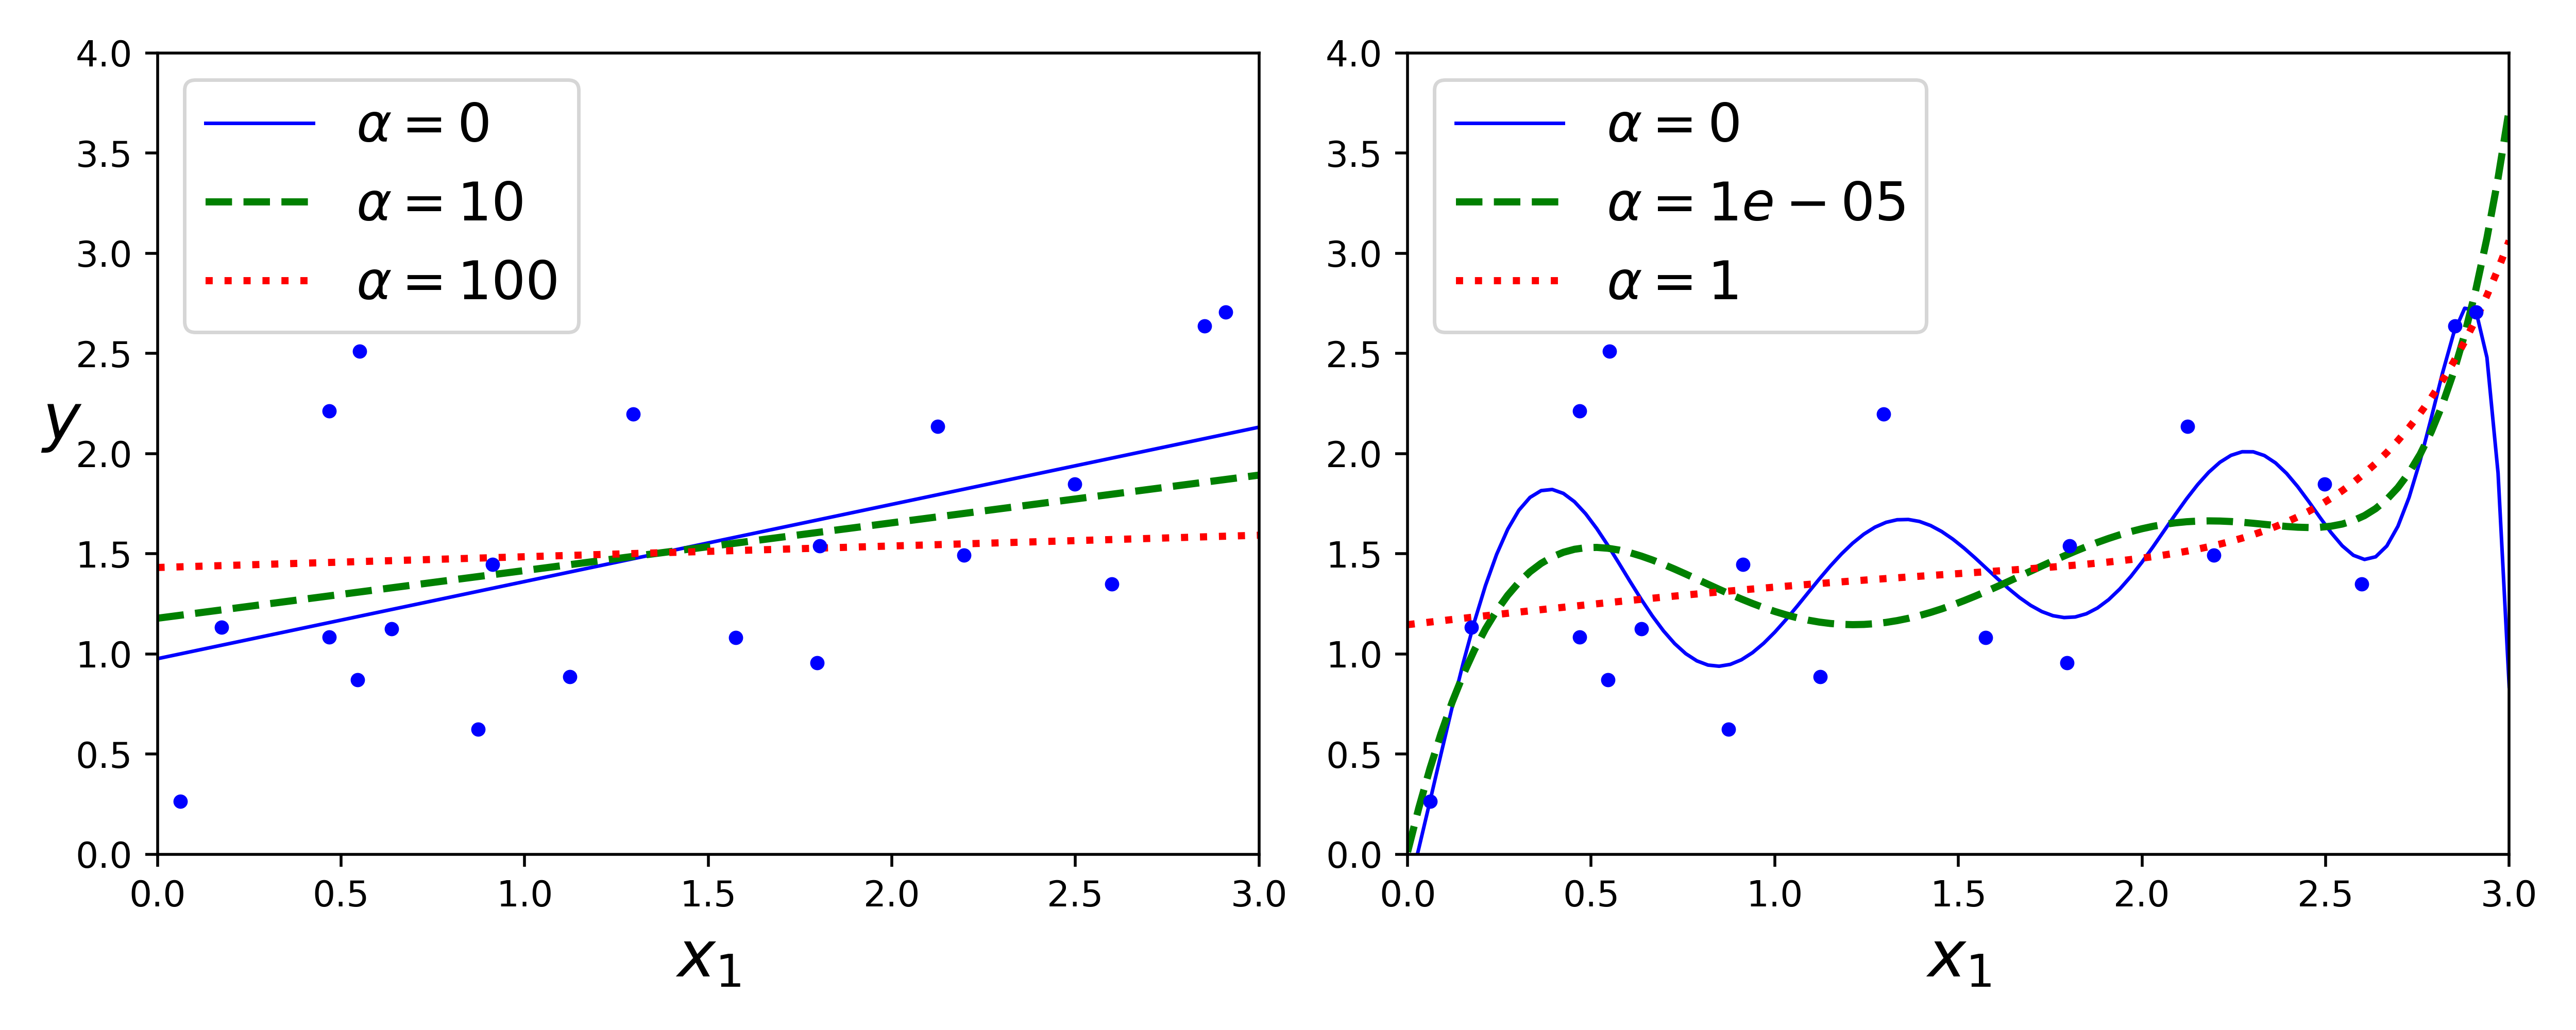
\includegraphics[width=12cm, height=7cm, keepaspectratio]{images/regularization_11.png}
\end{center}
\end{frame}

\begin{frame}{LASSO regresszió}
\begin{columns}
\begin{column}{.5\textwidth}
A LASSO (\textbf{L}east \textbf{A}bsolute \textbf{S}hrinkage and \textbf{S}election \textbf{O}perator) regresszió a ridge-hez hasonlóan egy büntetőkifejezés segítségével regularizálja az illesztett modellt.\par\medskip
Ebben az esetben a büntetőkifejezés nem a paraméterek négyzetének összege, hanem az abszolút értékének.
\end{column}
\begin{column}{.5\textwidth}
\begin{block}{A LASSO költségfüggvénye}
\[
J\left( \theta \right) = MSE\left( \theta \right) + \alpha \sum \left|\theta\right|
\]
Ahol: 
\begin{itemize}
	\item $MSE=\frac{1}{n} \sum_{i=1}^n \left( y_i - \hat{y}_i \right)^2$ az átlagos eltérés-négyzet
	\item $\sum \left|\theta\right|$ az $\ell_1$ norma büntetőkifejezés
	\item $\alpha$ a regularizáció mértékét adó együttható
	\item $\theta$ a paraméterek vektora
\end{itemize}
\end{block}
\end{column}
\end{columns}
\end{frame}

\begin{frame}{LASSO a gyakorlatban}
A LASSO a regularizáláció mellett elvégzi a jellemzőkiválasztás műveletét is. A felesleges paramétereket eliminálja, tehát $0$ értékeket ad nekik.\par\medskip
Az így létrejövő modellben kevés lesz a nem nulla súly. 
\begin{center}
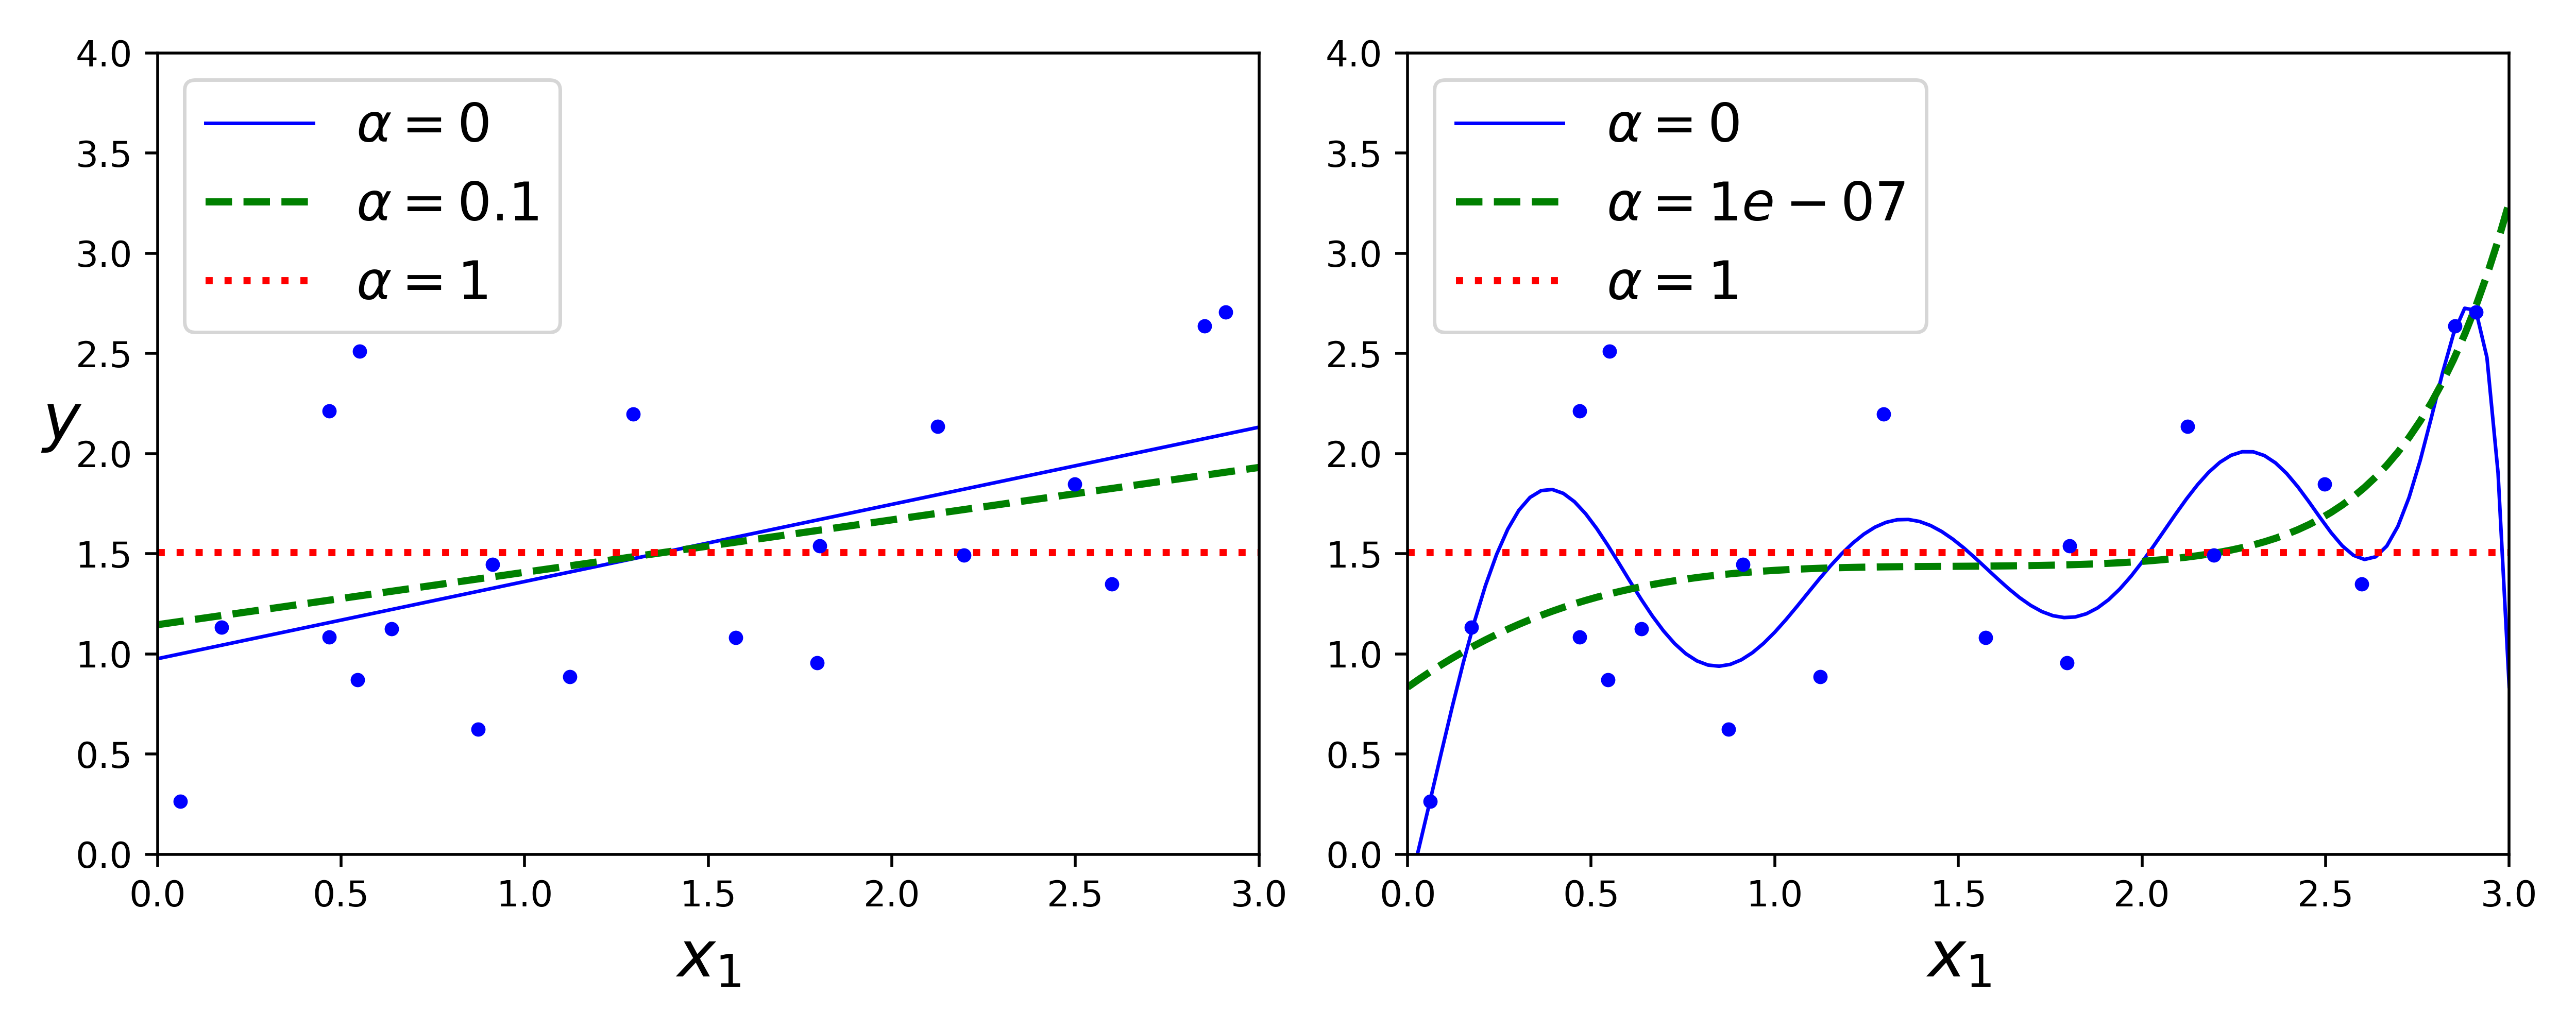
\includegraphics[width=12cm, height=7cm, keepaspectratio]{images/regularization_12.png}
\end{center}
\end{frame}

\begin{frame}{$\ell_1$ és $\ell_2$ norma}
\begin{columns}
\begin{column}{.5\textwidth}
A LASSO büntetőkifejezése az $\ell_1$ normát, a ridge pedig az $\ell_2$ normát használja. 
\begin{itemize}
	\item A LASSO jobban teljesít kevés független változó esetén
	\item A LASSO végez jellemzőkiválasztást
	\item A LASSO az egymással korreláló változók közül egyet hagy meg
	\item A ridge az egymással korreláló változókat együtt kezeli
	\item A ridge jobban teljesít, amikor minden független változó befolyásolja az outputot
\end{itemize}
\end{column}
\begin{column}{.5\textwidth}
\begin{center}
\includegraphics<1>[width=7cm, height=6cm, keepaspectratio]{images/regularization_13.png}
\includegraphics<2>[width=7cm, height=6cm, keepaspectratio]{images/regularization_14.png}
\end{center}
\end{column}
\end{columns}
\end{frame}

\begin{frame}{Gradiens ereszkedés LASSO és ridge regularizált függvényeken}
\begin{center}
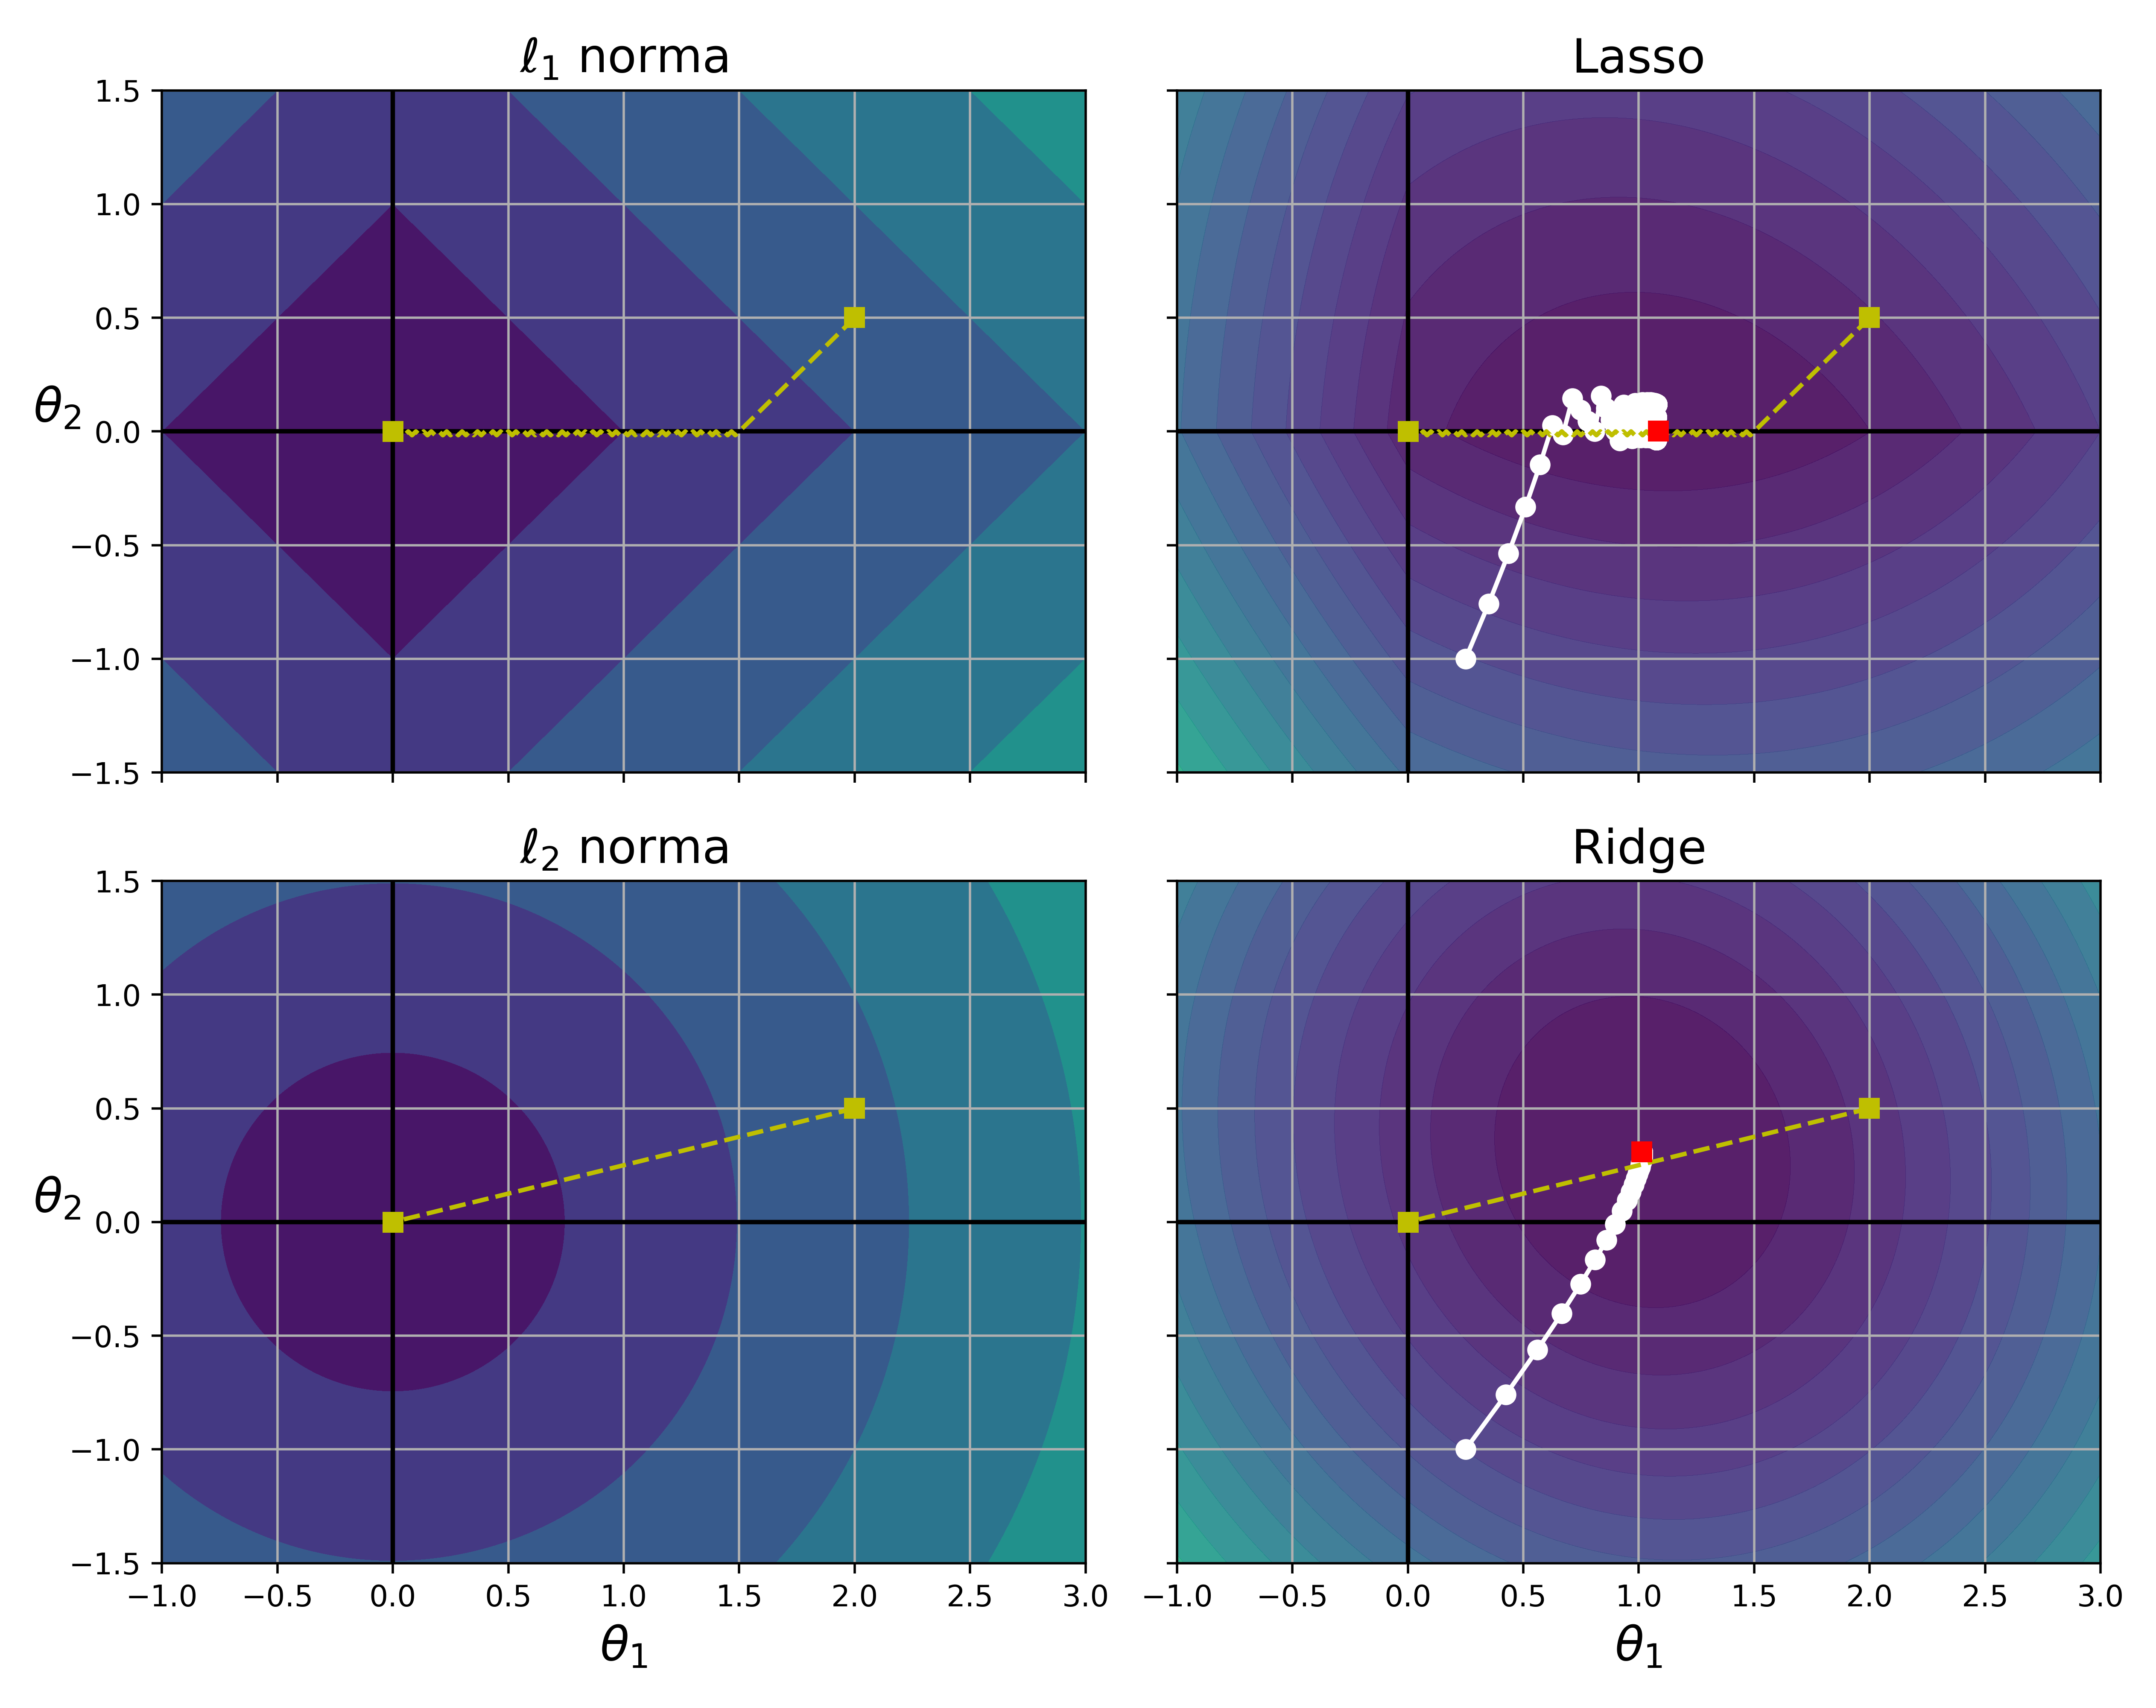
\includegraphics[width=14cm, height=7cm, keepaspectratio]{images/regularization_15.png}
\end{center}
\end{frame}

\begin{frame}{Elasztikus hálók [\href{https://www.geogebra.org/m/j9kh3ju2}{demo}]}
Az elasztikus háló egy \textbf{arányosságot definiál a LASSO és ridge modellek között}. A büntetőkifejezés egy keveréke a LASSO és ridge költségfüggvényeinek egy adott $r$ keverési arány szerint.\par\smallskip
Ha $r=0$ az elasztikus háló megegyezik a ridge modellel, ha $r=1$ akkor megegyezik a LASSO függvénnyel. 
\begin{block}{Az elasztikus háló költségfüggvénye}
\[
J\left( \theta \right) = MSE\left( \theta \right) + r \cdot \alpha \cdot \sum \left|\theta\right| + \left( 1-r \right) \cdot \alpha \cdot \sum \theta^2
\]
\begin{itemize}
	\item $MSE\left( \theta \right)$: Átlagos eltérés-négyzet
	\item $r \in \left[ 0, 1 \right]$: Keverési arány
	\item $\alpha$: Regularizációs együttható
\end{itemize}
\end{block}
\end{frame}

\section{Módszertan}

\begin{frame}
\tableofcontents[currentsection]
\end{frame}

\begin{frame}{Jellemző összevonás és kiválasztás}
\begin{columns}
\begin{column}{.5\textwidth}
\only<1>{\begin{block}{Jellemző összevonás}
Jellemzők összevonása során meglévő változók alapján új változók kerülnek létrehozásra valamilyen aggregációs függvény vagy más eljárás alapján pl. főkomponenselemzés.
\end{block}}
\only<2>{\begin{block}{Jellemző kiválasztás}
A jellemzők kiválasztása során változók közül eldobásra kerülnek azok, amelyekre nincs szükség a modellezés szempontjából valamilyen metrika szerint. 
\end{block}}
\end{column}
\begin{column}{.5\textwidth}
\begin{center}
\includegraphics<1>[width=7cm, height=7cm, keepaspectratio]{graphs/regularization_1.png}
\includegraphics<2>[width=7cm, height=7cm, keepaspectratio]{graphs/regularization_2.png}
\end{center}
\end{column}
\end{columns}
\end{frame}

\begin{frame}{Jellemzők kiválasztásának lehetséges módjai}
\begin{columns}
\begin{column}{.5\textwidth}
\only<1>{\begin{block}{Szűrés}
Nem tesztel adott algoritmust, csak egy módszertan szerint fontossági sorrendet definiál a változók között, és az egy küszöbérték alattiakat elveti.
\end{block}}
\only<2>{\begin{block}{Iteratív}
Specifikus modelleket kiértékel a jellemzők különböző részhalmazai szerint, majd azt választja ki amelyik a legjobb eredményt adja.
\end{block}}
\only<3>{\begin{block}{Beágyazott}
Minden technika ide tartozik, ami a tanítási fázisban jellemzőkiválasztást végez. Pl.: LASSO.
\end{block}}
\end{column}
\begin{column}{.5\textwidth}
\begin{center}
\includegraphics<1>[width=7cm, height=7cm, keepaspectratio]{graphs/regularization_3.png}
\includegraphics<2>[width=7cm, height=7cm, keepaspectratio]{graphs/regularization_4.png}
\includegraphics<3>[width=4cm, height=7cm, keepaspectratio]{graphs/regularization_5.png}
\end{center}
\end{column}
\end{columns}
\end{frame}

\begin{frame}{Korai leállás}
\begin{columns}
\begin{column}{.5\textwidth}
A korai leállás egy olyan technika gépi tanulásban amely \textbf{segít megakadályozni a túltanulást egy tanítási folyamat során}.\par\medskip
Ezáltal \textbf{leállítja a tanítást, amint a hálózat teljesítménye elkezd romlani}, vagy nem javul tovább a validációs adatkészleten.
\end{column}
\begin{column}{.5\textwidth}
\begin{center}
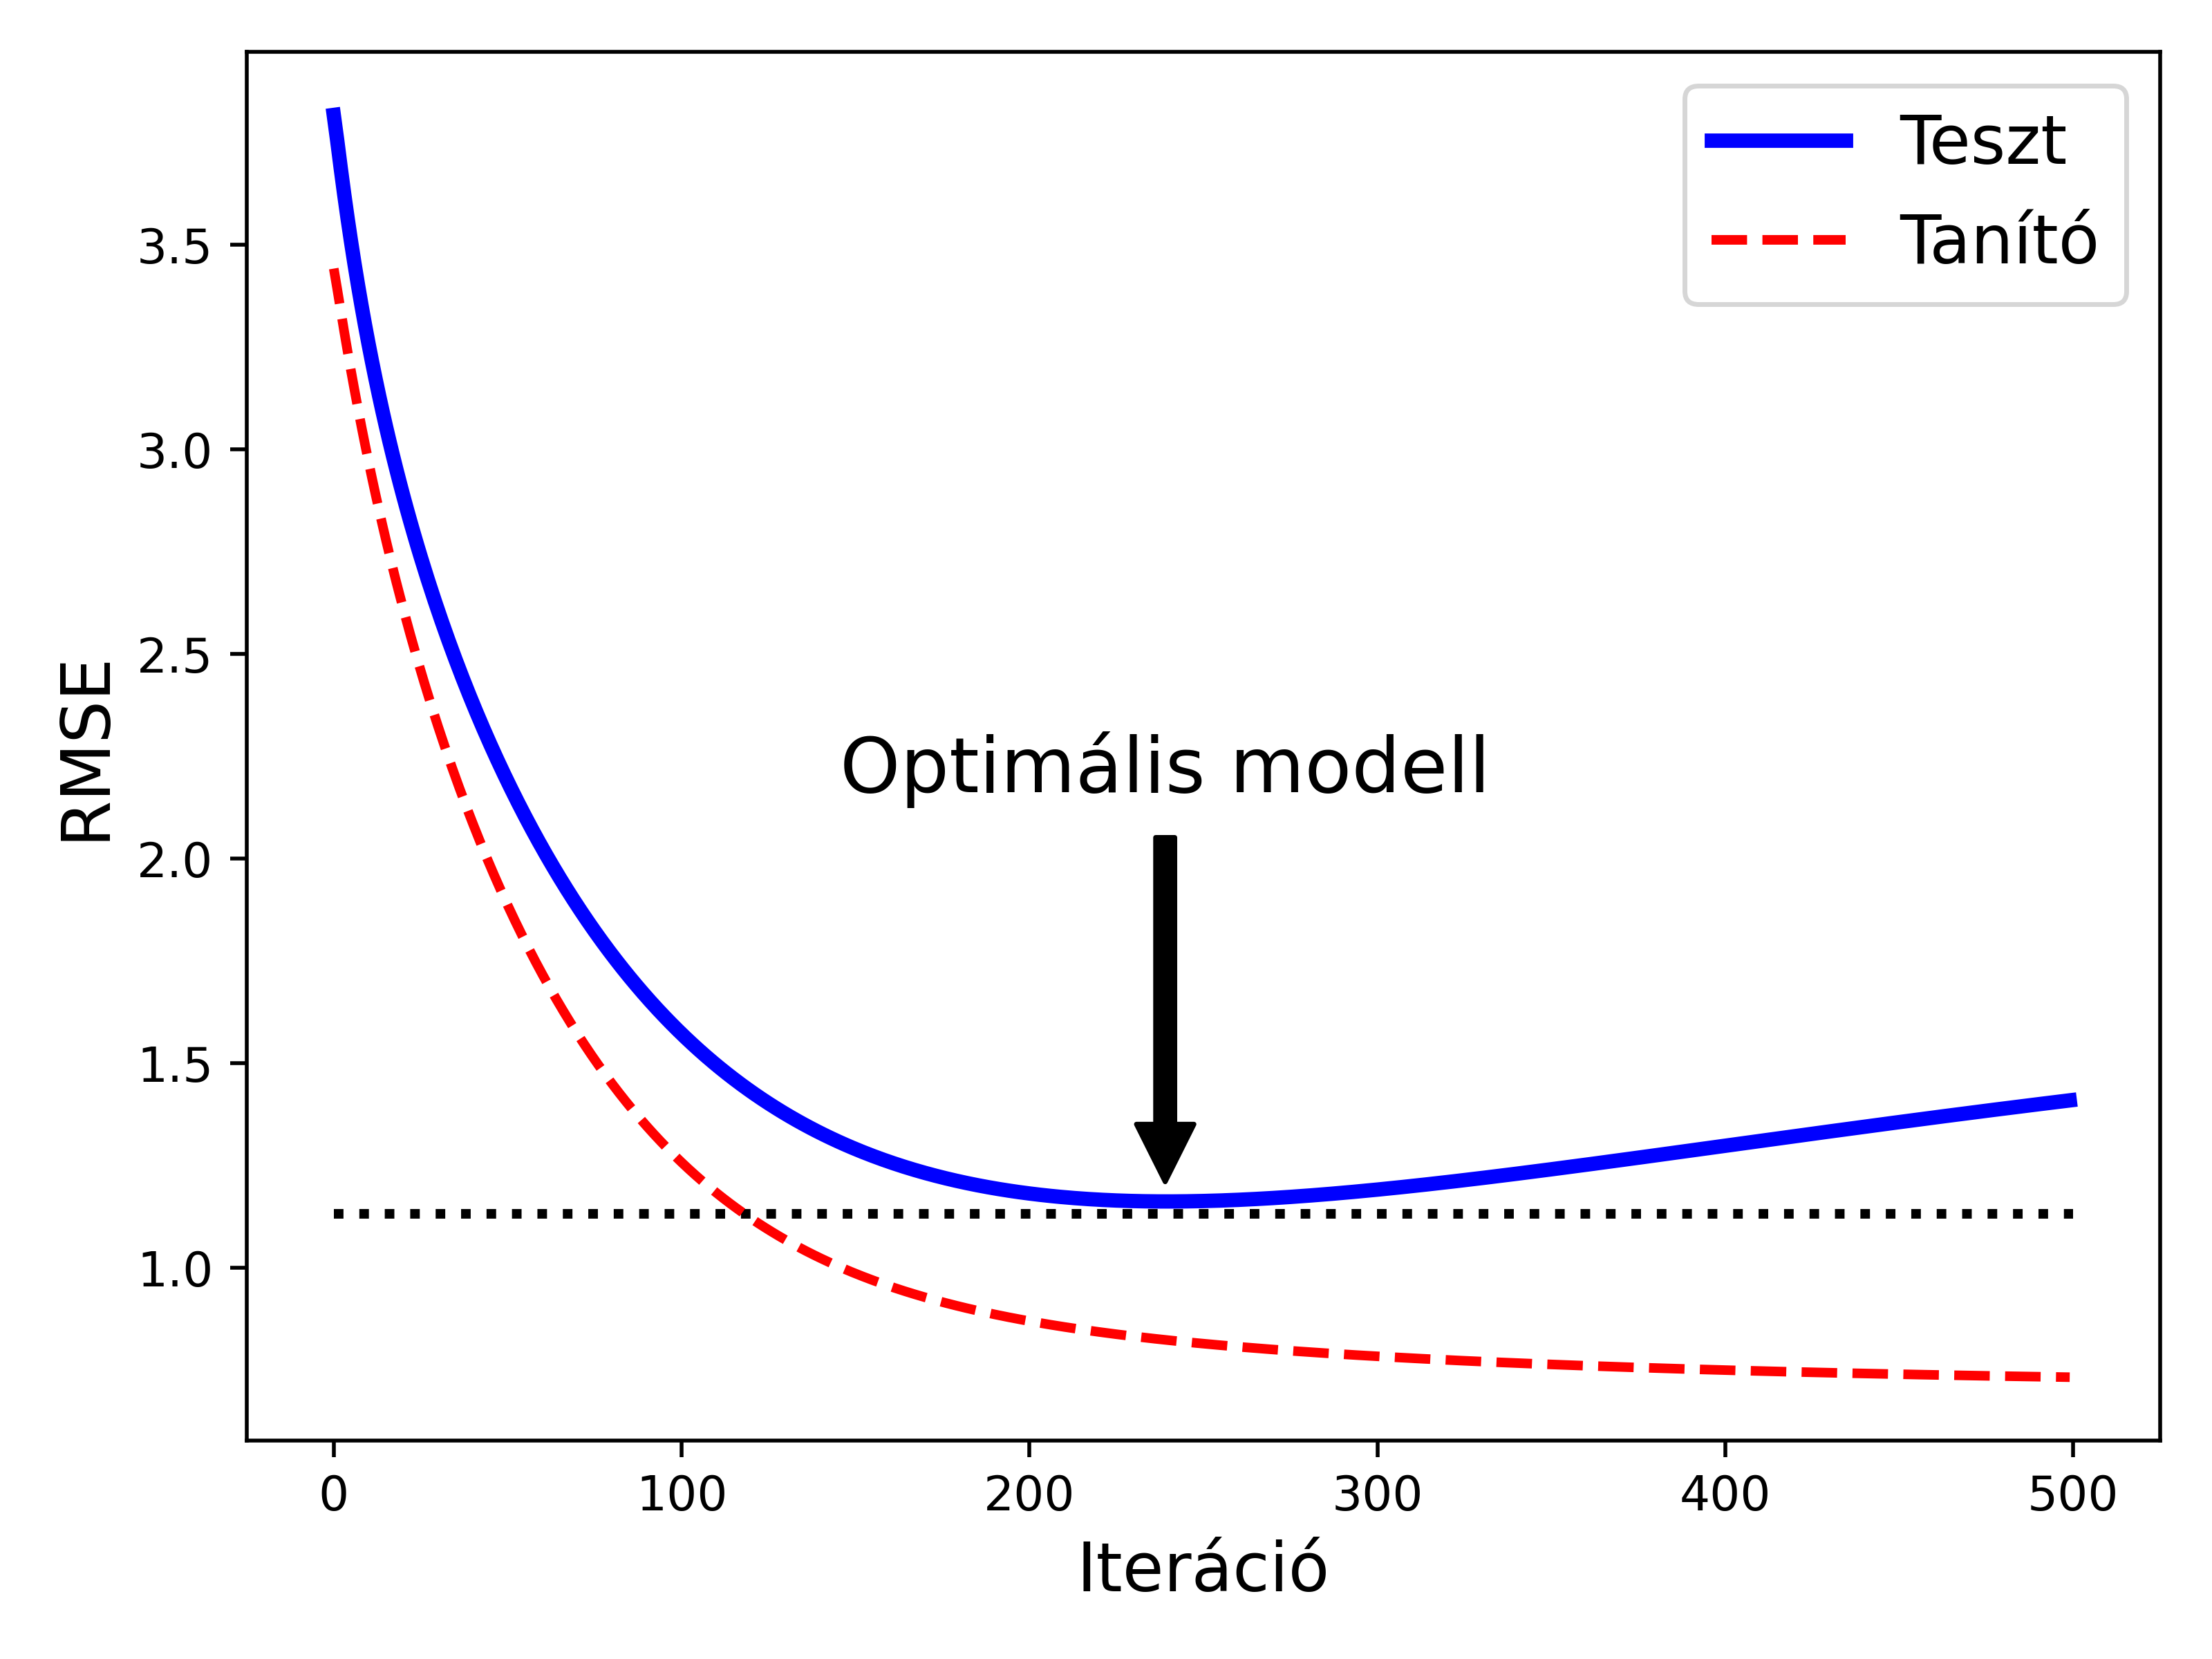
\includegraphics[width=7cm, height=7cm, keepaspectratio]{images/regularization_16.png}
\end{center}
\end{column}
\end{columns}
\end{frame}

\begin{frame}{$k$-hajtásos keresztvalidáció}
\begin{columns}
\begin{column}{.4\textwidth}
A technika az eredeti adatkészletet $k$ egyenlő részre osztja, \textbf{majd minden iterációban egy különböző részhalmazt használ tesztelésre, a többit pedig tanításra}.\par\medskip
Ez lehetővé teszi \textbf{a modell általánosító képességének pontosabb becslését}.
\end{column}
\begin{column}{.6\textwidth}
\begin{center}
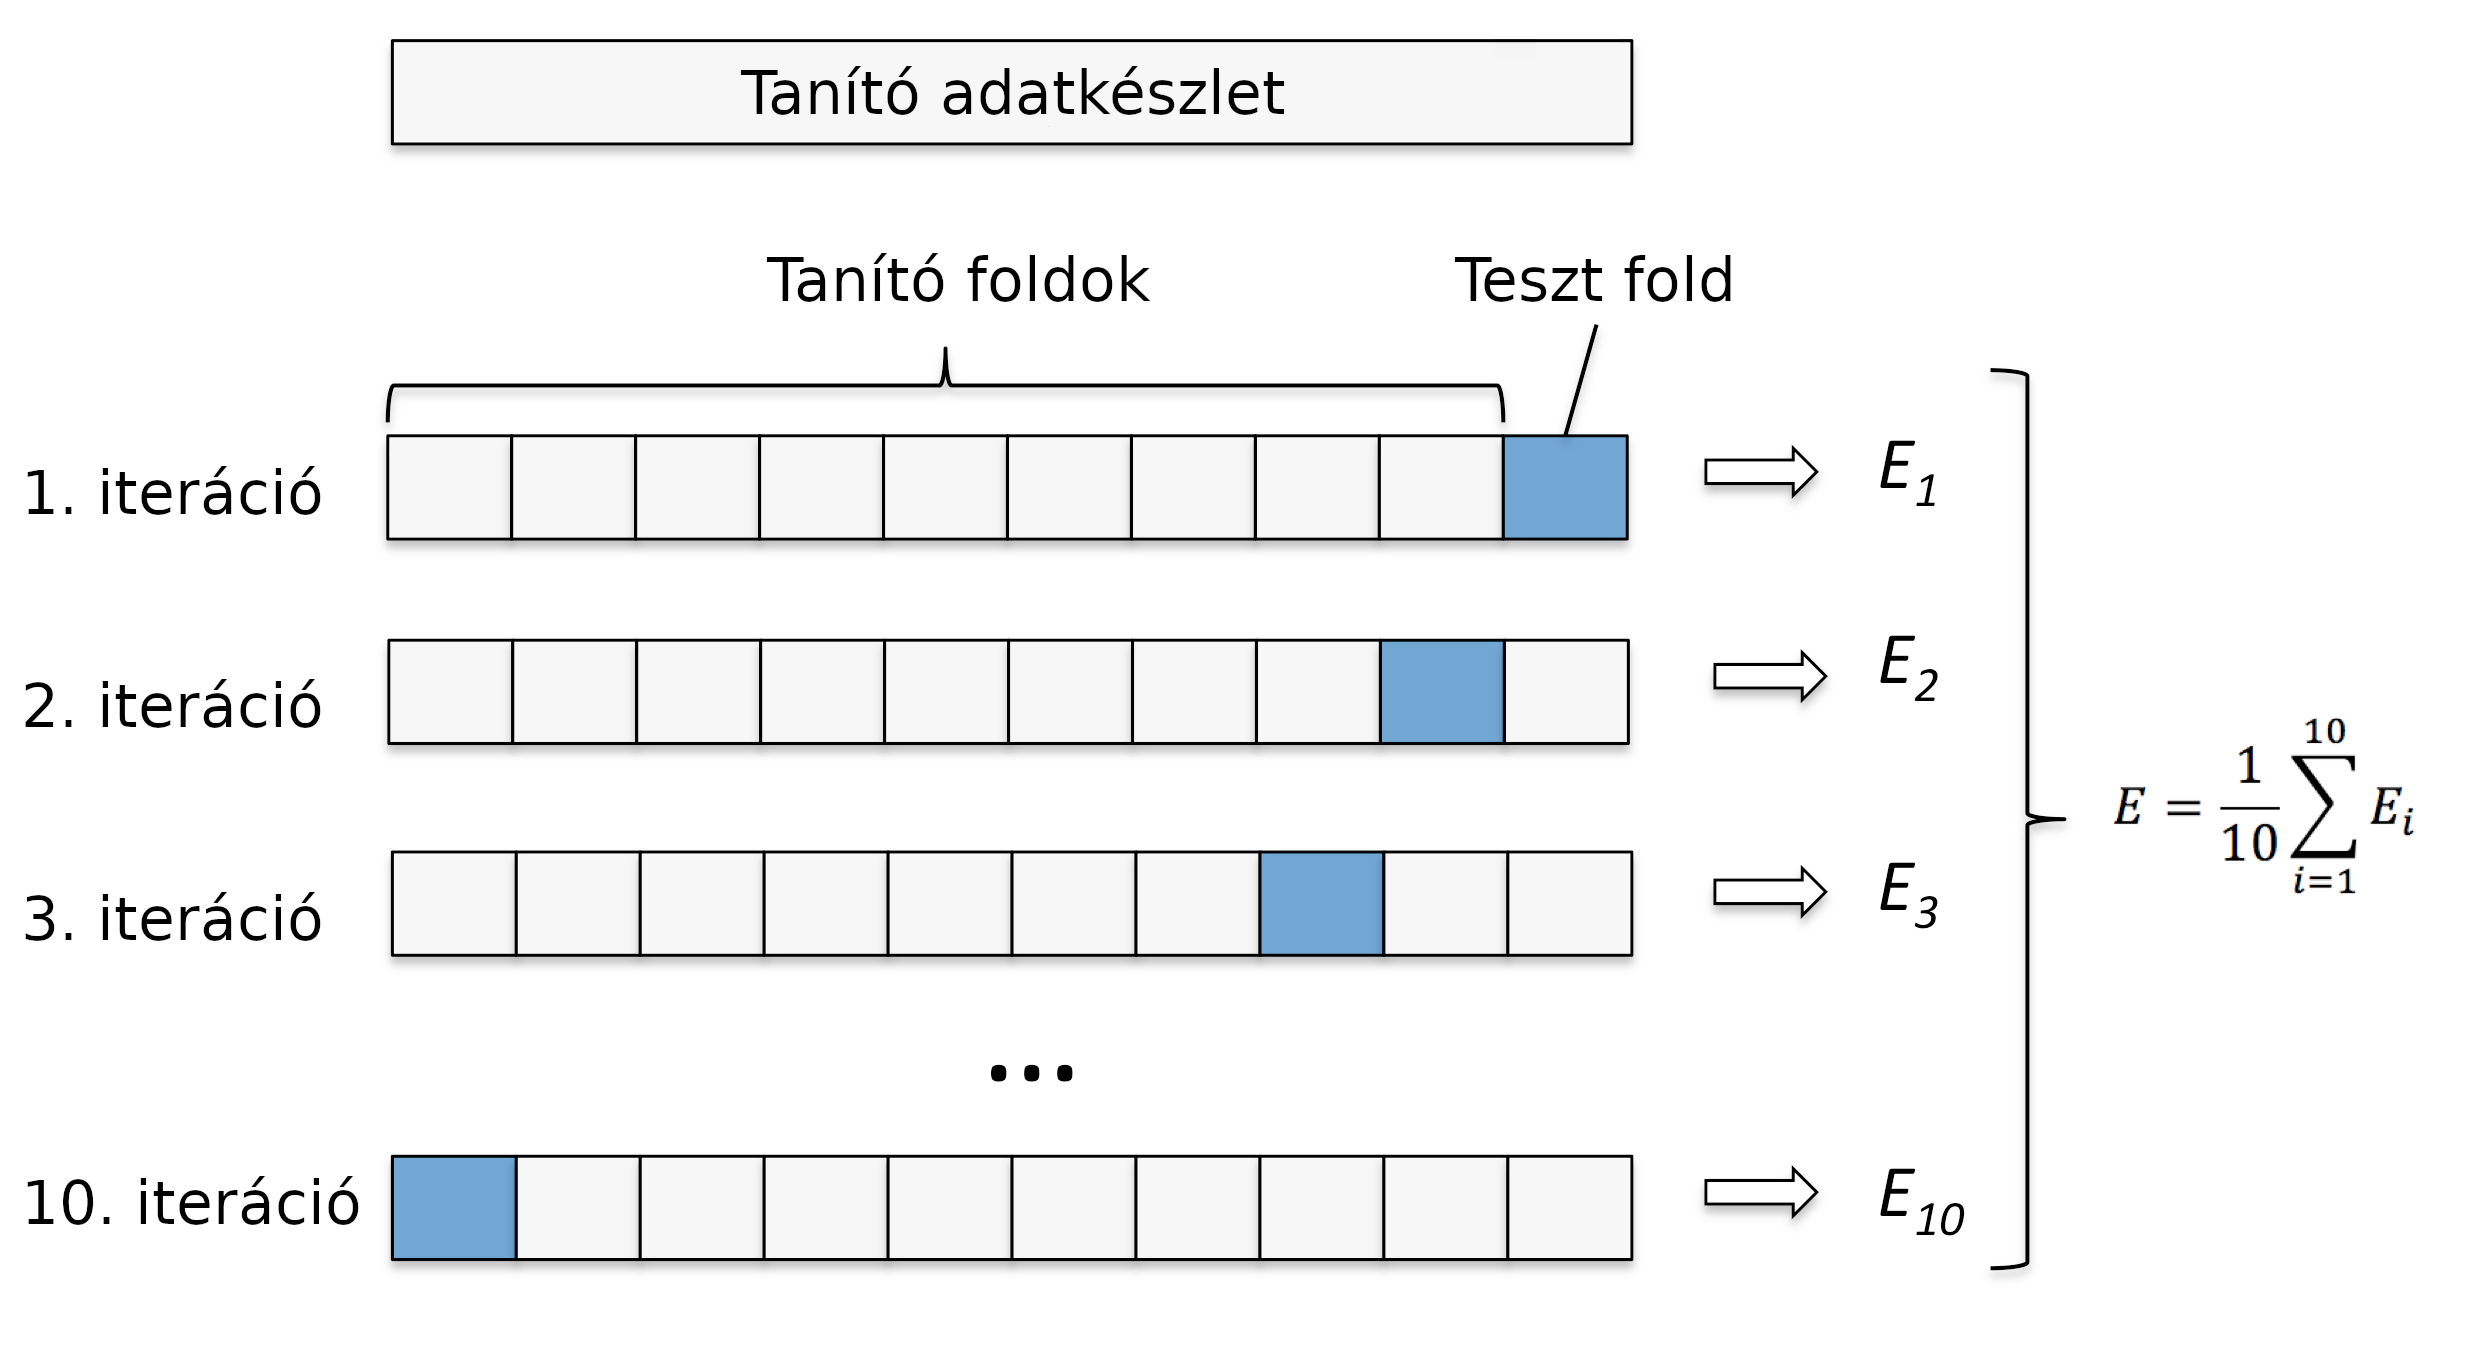
\includegraphics[width=9cm, height=9cm, keepaspectratio]{images/regularization_18.png}
\end{center}
\end{column}
\end{columns}
\end{frame}

\end{document}
















